%Use XeLaTeX
\documentclass[a4paper,10pt,]{report}
%
\usepackage{fontspec}
\setmainfont{Arial}
\usepackage{textgreek}
%
\newcommand\tab[1][0.5cm]{\hspace*{#1}}
%
\usepackage{geometry}
\geometry{a4paper, left=25mm, right=20mm, top=20mm, bottom=20mm}
\usepackage{changepage}
%
\usepackage{setspace}
%
\usepackage{parskip}
%
\usepackage{titlesec}
\setcounter{secnumdepth}{4}
\newcommand*{\justifyheading}{\raggedright}
	\titleformat{\chapter}
		{\normalfont\Large\bfseries\justifyheading}{\thechapter.}{1em}{} 
		\titlespacing{\chapter}{0pt}{0pt}{0pt}
		\titleclass{\chapter}{straight}

	\titleformat{\section}
  		{\normalfont\large\bfseries\justifyheading}{\thesection}{1em}{}
		\titlespacing*{\section}{0pt}{0pt}{0pt}
	\titleformat{\subsection}
  		{\normalfont\normalsize\bfseries\justifyheading}{\thesubsection}{1em}{}
		\titlespacing*{\subsection}{0pt}{0pt}{0pt}
         \titleformat{\subsubsection}
  		{\normalfont\normalsize\bfseries\justifyheading}{\thesubsubsection}{1em}{}
		\titlespacing*{\subsubsection}{0pt}{0pt}{0pt}
%
\usepackage{tocloft}
\renewcommand{\cfttoctitlefont}{\Large\bfseries}
\setlength{\cftbeforetoctitleskip}{-3em}
\setlength{\cftaftertoctitleskip}{2em}
%
\pagenumbering{arabic}
%
\usepackage{graphicx}
\graphicspath{/}
\renewcommand{\thefigure}{\arabic{figure}}
\renewcommand{\thetable}{\arabic{table}}
%
\usepackage{tikz}

%
\usepackage{enumitem}
%
\usepackage{amsmath}
\usepackage{amssymb}
\usepackage{pifont}
\newcommand{\xmark}{\ding{55}}
\newcommand{\cmark}{\ding{51}}

%
\usepackage{multirow}
\usepackage{array}
\usepackage{siunitx}
\sisetup{input-symbols = ()}

%
\usepackage{float}
\usepackage{epstopdf}
%
\usepackage{datetime}
\newdateformat{monthyeardate}{%
\monthname[\THEMONTH], \THEYEAR}
%
\usepackage{color}
\newcommand{\todo}[1]{\textcolor{red}{#1}}
%
\usepackage{natbib}
\bibliographystyle{agsm}
\usepackage{url}
%
\usepackage{scrextend}
%
\usepackage{chngcntr}
\counterwithout{figure}{chapter}
\counterwithout{table}{chapter}
\counterwithout{equation}{chapter}
%
\usepackage{changpage}
%
\renewcommand{\contentsname}{Table of Contents}
\renewcommand{\bibname}{References}
\usepackage{titletoc}% http://ctan.org/pkg/titletoc

\usepackage[nottoc,numbib]{tocbibind}

%-------------------------------------------------------------------------------------

\begin{document}

%--------------------------------------------------------------------------------------
\pagenumbering{gobble}
%---------------------------------------------------------------------------------------
\flushleft{\textbf{\Large{Summary}}}\\
\vspace{0.2cm}
Tropical tree species are shifting their ranges upslope in response to increasing temperature. As they move upslope, species are also likely to encounter changes in other environmental variables, including the biotic environment. Species are likely to differ in their ability to acclimate to these novel biotic conditions, with those of lower phenotypic plasticity experiencing increased stress at their range limits. Despite this, the majority of models predicting species range-shifts in response to climate change do not account for spatial variation in biotic environment.

This study investigated how seedlings of nine locally common neotropical tree species are responding to variation in seedling-seedling and adult-seedling competition, across their elevational ranges. Linear mixed models compared the strength and direction of relationships between competition variables and plant traits to determine: (a) whether competition effects cause variation in plant traits, and (b) how these effects compare to the effect of elevation. A recommendation is made on whether competition effects should be included in range shift models.

This study found that plant traits varied in response to above- and below-ground adult-seedling competition but not seedling-seedling competition. The effects of competition were smaller than elevation for all plant traits. Variation in plant traits across elevation was found to be species specific. Physiological stress decreased with elevation in 8/9 species. It is concluded that competition effects should be incorporated into future models predicting species range shifts in order to more accurately predict species range limitations, but that competition variables remain subordinate to abiotic environmental variables in these models.


\clearpage

\flushleft{\bfseries{\Large{Acknowledgements}}}\\
\vspace{0.2cm}
Firstly, I would like to thank Pippa Stone for organising much of the field season in Peru and for allowing me to be a part of such crucial research. Secondly, I thank Dr. Kyle Dexter and Dr. Isla Myers-Smith for their valuable advice regarding statistical analysis. Lastly I am deeply grateful to Rosamund Fitzmaurice for her constant support throughout the writing process.
\vspace{12cm}\\
\normalfont{\Large{\bfseries{Abbreviations}}}
\vspace{0.5cm}\\
\begin{tabular}{ l l l }
ABERG & = & Andes Biodiversity Ecosystem Research Group \\
adjR\textsuperscript{2} & = & Adjusted R-squared\\
AIC & = &Akaike Information Criterion\\
DBH &= &Diameter at Breast Height\\
F\textsubscript{v}/F\textsubscript{m} & = & Quantum efficiency of PSII \\
GLMM &=& Generalised Linear Mixed Model\\
ha & = & Hectare\\
ISI &= &Iterative Seedling Index\\
LAI &= &Leaf Area Index\\
LMM& = &Linear Mixed Model\\
m.a.s.l. & = & Metres above sea level\\
PAR& = &Photosynthetically Active Radiation\\
PSII & = & Photosystem II\\
$R_C^2$ & = & Whole model pseudo-r-squared\\
$R_M^2$ & = & Fixed Effect pseudo-r-squared\\
SD & = & Standard Deviation\\
SE & = & Standard Error of the mean\\
SPAD & = & Soil Plant Analysis Development (relative chlorophyll content)\\
UV-B & = & Ultraviolet light of wavelength 320-290 nm\\
VIF & = & Variance Inflation Factor\\
$W_i$ & = & Akaike weight\\


\end{tabular}


\clearpage
\onehalfspacing
\centering{\tableofcontents}
\clearpage
%---------------------------------------------------------------------------------------
\pagenumbering{arabic}
\setcounter{page}{1}
\raggedright
\chapter{Introduction}

\section{The Importance of understanding range shift patterns}
There is consistent evidence that rapid anthropogenic climate change is causing many species, across a wide range of taxa, to shift their distributions in space \citep{Hughes2000, McCarty2001, Walther2002, Parmesan2006, Loarie2009, Chen2011}. Within an ecosystem however, range shifts are not occurring equally across species, and will produce novel species assemblages in the future \citep{Hobbs2006}. Species specific range shift patterns will occur as the result of varying sensitivity to climate change caused by differences in ecology and evolutionary history \citep{Mooney2009}. The combination of novel species assemblages and novel abiotic conditions creates the potential for an increasing number of species to be less adapted to their environment. This may lead to reductions in local and regional species richness \citep{Colwell2008}, ecosystem functioning \citep{Bellard2012}, and ecosystem service provision \citep{Dobson2011, Isbell2011}. Climate induced species range shifts therefore add another mechanism by which anthropogenic change is contributing to a reduction in global diversity \citep{MillenniumEcosystemAssessment2005} and a homogenisation of community composition \citep{Dornelas2014} that is comparable to previous mass extinctions \citep{Barnosky2011}. It is therefore of paramount importance for future conservation management strategies to understand how species differ in their reaction to the novel environments they encounter. Given that the Earth is committed to a changing climate regardless of the effectiveness of greenhouse gas emission mitigation \citep{IPCC2013}, the need for contingency plans is even more important.

%MORE ON THE POTENTIAL RESULT OF RANGE SHIFTS?

Previous studies have demonstrated that species' success over the coming century will be largely determined by their ability to respond to changing temperatures \citep{Colwell2008, Chen2011, Feeley2012}. Responses may occur either in the form of adaptation, \textit{i.e.} changes in phenology, physiology and morphology, or through range shifts over space as species track changing temperatures \citep{Bellard2012}. As well as the effect of temperature, previous studies have drawn attention to the biotic environment as a potential driver of species specific range-shift dynamics \citep{Ettinger2013,Araujo2007,Meier2010,VanderPutten2010,Wisz2013}.

The effects of biotic interactions have been largely ignored in previous range shift models, in the belief that they play a small role in limiting species ranges compared to abiotic environmental change (Pearson \& Dawson 2003, and references therein). There is little evidence to specifically suggest this is the case however \citep{Araujo2007}. There is robust evidence of the importance of various aspects of the biotic environment on population dynamics, including soil biota effects \citep{Wardle2004, VanGrunsven2010}, predation \citep{Hillyer2010}, competitive interactions \citep{Freckleton2009}, and mutualisms \citep{Meier2010}. However, little of this knowledge has been included in providing a mechanistic understanding of how biotic interactions may influence range shifts under climate change \citep{Araujo2007}. By understanding how species are affected physiologically by the biotic environment and how species adapt their morphology, more accurate and precise predictions of future range shifts can be made \citep{Feeley2010, Feeley2012}. %Ed comment
%
This study aims to partly fill this knowledge gap by measuring plant trait responses to competitive interactions, in order to assess whether models predicting range shifts should include such parameters.

\section{The role of biotic interactions}
Species ranges shift at different rates in response to climate change \citep{Walther2002}. As such, the relative overlap of different species' ranges is likely to change as climate change progresses, producing novel species assemblages. In forests, biotic interactions are often strong and species turnover occurs over short distances, primarily due to dispersal limitation and vertical stratification of forest habitat \citep{Condit2002}. Thus, the creation of novel species assemblages will lead to marked changes in competition among plants for resources such as light, nutrients, water and space \citep{Schweiger2008}. Trees are some of the slowest taxa to migrate in response to climate change due to their long life-span and sessile nature. Thus, trees will be affected by biotic interactions more than other taxa as they fail to track changes in climate at a suitable rate \citep{Wisz2013}. 

\citet{Araujo2007} compared the results of >600 studies and found that the inclusion of biotic interactions significantly increased the explanatory power of species range shift models. This trend was seen even at large scales where biotic interactions are expected to play a minor role compared to climate \citep{Davis1998}. Similarly, \citet{Gilman2010} found that biotic interactions affect communities at a range of spatial scales. Biotic interactions caused changes in individual fitness at the local scale, while at the regional scale they found changes in community structure. Unsurprisingly, range shift models that only include direct abiotic drivers of range shifts have often produced inaccurate predictions, with many becoming significantly better when biotic interactions are included \citep{Heikkinen2007}.

\section{Bioclimatic envelope models}
The majority of attempts to predict the spatial response of species to climate change have relied on bioclimatic envelope modelling \citep{Pearson2003}. Bioclimatic envelopes are constructed from correlations between present species spatial boundaries and observed environmental conditions within those boundaries, then projected into the future under different climate change scenarios to predict how species boundaries will change \citep[e.g.][]{Berry2002, Peterson2002, Thuiller2005, Araujo2006} \citep{Sinclair2010}. These models make a number of over-simplifications and assumptions however, leading to criticisms over their accuracy \citep{Pearson2003}.

Basic bioclimatic envelope models assume that the breadth of the realised niche (observed spatial range) equals that of the fundamental (bioclimatic envelope) niche \citep{Jump2005, Hoffmann2011}. This assumption is challenged by studies which demonstrate that the realised niche is often smaller than the fundamental niche, owing to biotic interactions with other species \citep{Davis1998, VanderPutten2010, Ettinger2011}. Furthermore, bioclimatic envelope models assume that species respond instantaneously to climate change and that this change is equal in across all individuals of a species. This ignores potential lag effects caused by dispersal limitation, adaptive capacity limits, and intra/interspecific variation of these constraints \citep{Jackson2010, McLaughlin2012}. Currently, the accuracy of bioclimatic envelope models is limited by a paucity of data regarding the effects of non-climatic range shift rate controls on individuals and populations \citep{Wiens2011}. Furthermore, it is inadequate to add biotic range shift controls as a simple exponent or constant to be added to range shift models, as biotic effects interact with each other in complex ways and species respond heterogeneously to them \citep{Parmesan2006, Moritz2008, Doak2010, Feeley2011}. By adding biotic interactions such as competition to bioclimatic envelope models, the realism and accuracy of these models could be increased \citep{Araujo2007}.

\section{Tropical elevational gradients as natural laboratories}
Tropical forests form an ideal system in which to investigate effects of the biotic environment over species ranges. Compared with temperate species, tropical species are more sensitive to changes in temperature due to a lack of seasonal temperature variation \citep{Janzen1967, Ghalambor2006, McCain2009}. Species found in the tropics are therefore more likely to shift their ranges in response to climate change than those found in other biomes.

Elevational gradients in the tropics are more likely to exhibit changes in species ranges compared to topographically uniform areas. Much of the migration in the tropics will occur across altitude rather than across latitude as tropical forests feature a relatively strong elevation-temperature gradient compared to other latitudes and have a low rate of temperature change with latitude \citep{Malhi2010}. This means that cooler regions are much further away latitudinally than altitudinally in the tropics.

The neotropical forest spanning the Eastern flanks of the Andes, the region investigated in this study, is expected to be particularly sensitive among tropical regions to changes in climate. Palaeological records show a strong correlation between previous climate change and changes in forest composition \citep{Bush2004, Urrego2010}. Furthermore, the rate of regional temperature increase as a result of climate change in this region currently exceeds that of the global average \citep{Vuille2000}, range shifts are therefore expected to become apparent here before other tropical regions. It is hoped therefore, that studies conducted in this region will form a strong knowledge base for predicting range-shifts elsewhere.

Tropical forests are under-studied by investigations aiming to understand global ecological patterns \citep{Malhi2010}. This is despite tropical forests playing an important role in the global carbon cycle \citep{Davidson2012} and contributing largely to global biodiversity trends \citep{Gaston2000}. Tropical studies are often marred by the consequences of extreme weather, a hostile biotic environment, and the inaccessibility of remote locations. Thus, studies such as this one, which focus specifically on tropical will make an important contribution to a growing body of evidence on the functioning of tropical ecosystems. Specifically, this study focusses on a high elevation tropical ecosystem, which are understudied compared to other tropical ecosystems \citep{Bubb2004}.

\section{This study, objectives and rationale}
This study investigates the acclimatory response of seedlings of evergreen neotropical tree species to variation in competition intensity across their elevational ranges. The competition variables measured are proxies for adult-seedling above- and below-ground competition and seedling-seedling competition. The study focusses on an elevational migration corridor in the Peruvian Andes along which tree species ranges are known to be shifting upslope \citep{Feeley2011}. Variation in seedling physiological and morphological traits in response to variation in competition intensity is used to evaluate whether these biotic interactions have the potential to affect future range-shift dynamics (RQ1). The strength of the competition-trait relationship is then compared to the general elevation-trait relationship to determine the relative importance of variation in competition intensity in influencing future range shifts (RQ2). a recommendation will be made as to whether competitive interactions should be included in future range-shift models in the tropics.

The plant traits measured in this study are both morphological and physiological. Analysis of chlorophyll fluorescence assesses the photosynthetic performance of individuals, with a reduced photosynthetic efficiency interpreted as evidence of plant stress \citep{Ashraf2013}. Leaf chlorophyll content is also measured. Decreased leaf chlorophyll content is also interpreted as a sign of plant stress, being associated with senescence and nutrient deficiency \citep{Gitelson2003}. Decreased chlorophyll content (chlorosis) can be caused by acclimation to a more intense light regime, as a result of a deficiency in available soil nitrogen, or as a result of plant stress or senescence \citep{Ashraf2013}. Variation in morphological plant traits: leaf thickness, leaf area, stem volume and the leaf:height ratio provides an insight into the ability of individuals to acclimate to different environmental conditions, thus showing whether a species is sensitive to changes in the environment.

%The results from this study are used to evaluate whether competitive interactions should be included in future models predicting upslope migration trends of tree species in this locality, and tropical tree species in general.

%This study focusses on the role of competitive interactions in determining plant traits and whether this response to the biotic environment forms part of the overall response to elevation or contrasts it (RQ1). The study also clarifies whether the biotic environment does in fact vary over elevation and whether neotropical tree plant traits are responding to elevation (RQ2). Additionally, this study aims to confirm whether plant trait responses to elevation are species specific. The primary objective of this study is to elucidate whether competitive interactions significantly influence plant traits along this elevational gradients. 
\clearpage
\subsection*{Research questions \& null hypotheses}
\textbf{RQ1:} Do competition variables explain variation in plant traits?\\
\vspace{3 mm}
H\textsubscript{n1}: Competition variables explain no variation in plant traits.\\
\vspace{2 mm}
H\textsubscript{n2}: No combination of competition variables and/or elevation predicts variation in plant traits better than elevation used in isolation.\\
\vspace{4 mm}
\textbf{RQ2:} To what extent do competition variables and plant traits vary across elevation and among species?\\
\vspace{3 mm}
H\textsubscript{n3}:  Competition variables do not vary with elevation.\\
\vspace{2 mm}
H\textsubscript{n4}:  Within each species, plant trait variables do not vary with elevation.\\
\vspace{2 mm}
H\textsubscript{n5}: The nature of the relationship between plant traits and elevation does not vary with species.\\

\chapter{Methods}
\section{Study site}
Measurements were conducted across 10 permanent 1 ha closed canopy forest plots in the Kos\~{n}ipata Valley of Man\'{u} National Park, Peru (-13\textdegree N, -71\textdegree W, Figure \ref{fig:sites}, Table \ref{table:sitechar}). The Kos\~{n}ipata Valley has been identified as a potential migration corridor for lowland species to migrate to higher elevations in response to temperature increase \citep{Feeley2011}. Plots are situated between 400 and 3200 m.a.s.l. along this migration corridor (Table \ref{table:sitechar}, Figure \ref{fig:range_plot}). The plots form part of a larger plot network established by the Andes Biodiversity and Ecosystem Research Group (ABERG) in 2003 \citep{Malhi2010, Girardin2013a}.


 \begin{figure}[htbp]
 \centering
 \includegraphics[scale=0.5]{Sites.png}
 \caption{Maps showing the location of the study area and plot locations. \textbf{(A)} The site location within Peru with elevation shading, showing the proximity to Man\'{u} National Park (white area). \textbf{(B)} The location of the 1 ha plots within the Kos\~{n}ipata Valley. \textbf{(C)} An enlargement of the Trocha Union and San Pedro plot groups. Red crosses indicate plot location, white lines in maps (B) and (C) indicate roads, text labels in (B) and (C) are plot codes, dark green areas in (B) and (C) denote the bounds of Man\'{u} National Park.}
 \label{fig:sites}
 \end{figure}
 
% Add the SD / SE for some of the values, Add footnotes for sources of information
\begin{table}[H] \centering 
  \caption{Site characteristics for each 1 ha plot sampled in this study. `NA' no data available. Adapted from \citet{Whitaker2014}.} 
  \label{table:sitechar}
\begin{minipage}{\textwidth}
	\centering
\begin{adjustwidth}{-0.5cm}{-0.5cm}
\begin{center}
\begin{tabular}{@{\extracolsep{0pt}} rSSrcS[table-number-alignment=center, separate-uncertainty=true, table-figures-uncertainty=1, table-figures-decimal=1,table-figures-integer=1]cccccc} 
\\[-1.8ex]\hline 
\hline \\[-1.8ex] 
Site & {Latitude} & {Longitude} & {Elevation} & Annual  & {Mean Annual}  & Slope & Total & Total & Soil \\
 Code & {(\textdegree)} & {(\textdegree)} & {(m.a.s.l.)} & Precipitation & {Air Temperature} & (\textdegree) & N (\%)  & C (\%)  & pH  \\
 & & & & (mm year\textsuperscript{-1}) & {$\pm$ SD (\textdegree C)} & & & & \\
\hline \\[-1.8ex] 
PA400 & -12.655 & -71.234 & 406 &NA & NA & NA & NA & NA & NA \\ 
PA800  &-12.639 & -71.274 & 822& NA & NA & NA & 15.6 & 3.4 & NA \\ 
VC & -12.869 & -71.406 & 861 & 3,087 & 20.7 \pm 0.1 & NA & 16.0 & 1.5 & 3.9 \\ 
SP1500 &-13.049 & -71.536 & 1,497& 2,631 & 17.4 \pm 1.5 & 22.7 & 10.5 & 1.0 & 4.1 \\ 
SP1750 &-13.047 & -71.543 & 1,770& 2,631 & 15.8 \pm 1.3 & 40.1 & 26.0 & 1.9 & 4.3 \\ 
TRU08 & -13.070 & -71.556 & 1,839& 2,472 & 16.0 \pm 1.3 & 41.8 & 31.0 & 2.0 & 4.3 \\ 
TRU07 & -13.074 & -71.560 & 2,135& 1,827 & 14.9 \pm 1.1 & 18.0 & 37.0 & 2.1 & 4.0 \\ 
TRU06 &-13.080 & -71.566 & 2,281& NA & NA & NA & NA & NA & NA \\ 
TRU04  & -13.106 & -71.589 & 2,733&2,318 & 11.1 \pm 1.0 & 21.4 & 28.5 & 1.8 & 3.9 \\ 
TRU02  &  -13.111 & -71.604 & 3,213&NA & 8.9 \pm 1.0 & 11.8 & 44.5 & 2.6 & 3.8 \\ 
\hline \\[-1.8ex] 
\hline\\
\end{tabular} 
\centering
\end{center}
\end{adjustwidth}
\end{minipage}
\centering
\end{table}

The research area has a mean annual temperature range of \textasciitilde 12 \textdegree C, with an adiabatic lapse rate of 4.94 \textdegree C km\textsuperscript{-1},  from 20.7 $\pm$ 0.02 \textdegree C (mean $\pm$ standard deviation) (VC, 861 m.a.s.l.) to 8.9 $\pm$ 1.0 \textdegree C (TRU02, 3213 m.a.s.l.) \citep{Whitaker2014}. Annual precipitation ranges from 1700 - 3087 mm year\textsuperscript{-1}, with a hump-shaped distribution peaking at 1000 m.a.s.l., between SP1500 and VC. Despite low precipitation at higher elevations, sites are rarely moisture limited, due to limited evapotranspiration and frequent fog deposition within the cloud immersion zone, which extends from \textasciitilde 1500 to 3020 m.a.s.l. \citep{Weg2010}. 

Average soil temperature ranges from \textasciitilde27 $\pm$ 0.3 \textdegree C (mean $\pm$ SD) in PA400 to \textasciitilde 12 $\pm$ 0.3 \textdegree C in TRU04 (Figure \ref{fig:temp_mois_fit}a). Soil moisture content ranged from 2-75\%, showing no relationship with elevation (Figure \ref{fig:temp_mois_fit}b). Instead, micro-site effects reflecting geomorphological situation (proximity to run-off channels, rocky outcrops etc.) are likely to be the principal controls on soil moisture content \citep{Moser2008, Girardin2010}.  

The elevational gradient encompasses several complete ecosystem turnovers, with lowland tropical rainforest (<800 m.a.s.l.), followed by pre-montane (800-1200 m.a.s.l.), lower montane (1200 - 2200 m.a.s.l.) and upper montane (2200 - 3400 m.a.s.l.) cloud forest \citep{Girardin2010}. Plots between 1500 and 3020 m.a.s.l. (SP1500, SP1750, TRU08, TRU04) are frequently immersed in cloud, having structural features of cloud forests (short stature trees, dense crowns, twisted branches). All plots were originally sited with the aim of reducing within plot heterogeneity in terms of forest structure, geological substrate and topography (Girardin et al. \citeyear{Girardin2013b}a). Additionally, all montane plots (SP1750 - TRU02) were sited along a ridge-top; this reduces variation in non-elevationally dependent abiotic environmental variables within each site which are known to significantly impact montane forest dynamics, such as wind speed and aspect (Girardin et al. \citeyear{Girardin2013a}b). Measurements were taken between July and August 2015, prior to the start of the autumn rainy season \citep{Garreaud2009}. 
 
\section{Species}
Nine tree species were chosen for comparison from a range of 1635 identified species found in the plots. Species were selected according to their contrasting ranges (Figure \ref{fig:range_plot}), differences in migratory pattern of their genus \citep{Feeley2011}, and because they are dominant species across their ranges (ABERG, unpublished data, Appendix VI). Despite having no quantitative range shift prediction information, \textit{Iriartea deltoidea} and \textit{Dictyocaryum lamarckianum} were included in order to observe potential differences between monocot and dicot species, as both are monocots. Both \textit{I. deltoidea} and \textit{D. lamarckianum} are large-seeded palm species, as such, they are expected to be migrating upslope, similar to other large-seeded palms \citep{Hillyer2010}. Seedlings of \textit{Myrcia} spp. are difficult to reliably identify to species in the field and were thus sampled as a composite of three potential species: \textit{Myrcia splendens}, \textit{M. fallax}, and \textit{M. rostrata}, referred to as \textit{Myrcia} spp.. Species are referred to by two letter codes (AV, CR, etc.) hereafter (Table \ref{table:speciesnumseed}).\\


\begin{figure}[H] 
   \centering
   \includegraphics[scale=0.5]{Range_plot.png} 
   \caption{Elevational ranges of species sampled ($\blacksquare$), elevations of the 10 plots sampled (grey dashed lines) with plot names on the right side, and sampling locations of each species indicating upper (\tikz\draw[blue,fill=blue] (0,0) circle (.5ex);), central (\tikz\draw[green,fill=green] (0,0) circle (.5ex);) and lower (\tikz\draw[red,fill=red] (0,0) circle (.5ex);) elevation sample locations. Species show contrasting elevational ranges and contrasting range sizes. See Table \ref{table:speciesnumseed} for species codes and Table \ref{table:sitechar} for plot characteristics.}
   \label{fig:range_plot}
\end{figure}


\section{Sampling strategy}
Species were sampled in three plots, as close to the top, centre, and bottom of their elevational ranges as possible (Figure \ref{fig:range_plot}), to allow within species comparisons along each species range. \textit{D. lamarckianum} was sampled at only the top and bottom of its range due to the relative location of plots along its range. \textit{C. revoluta} was sampled in both TRU08 and SP1 due to a paucity of identifiable seedlings in SP1. \textit{I. deltoidea} seedlings could not be located in SP2 despite its range extending above this elevation.

In each of the three plots per species, a maximum of 10 seedlings were opportunistically sampled. Seedlings were used as they were easy to locate and measure, not requiring the use of tree climbing equipment as with adult trees. Additionally, seedlings are believed to be a crucial developmental stage with high mortality, being particularly sensitive to environmental stressors and more likely to show clear signs of stress \citep{Ettinger2013}. Seedlings were defined as \textless 1 m in height and bearing no woody parts.

Epiphytes and individuals connected by stolons or rhizomes to larger individuals were not sampled as these individuals may draw nutrients from their parent plant, invalidating correlations between observed plant traits and environmental variables. Seedlings with a minimum of two fully-expanded leaves and no visible signs of damage or herbivory were sampled to reduce sources of unknown bias in physiological measurements. To eliminate potential spatial pseudo-replication, only seedlings more than 5 m apart were sampled. This ensured that competition were independent and did not overlap, and seedlings were unlikely to be competing with each other \citep{Paine2008}. Within a cluster of seedlings, the seedling to be measured was chosen at random by assigning each seedling a number and using a random number table, reducing human bias. Due to the spatial distribution of seedlings and the overall abundance of accessible seedlings, it was not possible to sample 10 seedlings per plot for some species (Table \ref{table:speciesnumseed}).

\begin{table}[H] 
\centering 
  \caption{The number of seedlings sampled at each sample plot for each species and the species codes used throughout the report.} 
  \label{table:speciesnumseed} 
\begin{tabular}{@{\extracolsep{5pt}} lSSS} 
\\[-1.8ex]\hline 
\hline \\[-1.8ex] 
Species Name  & {Bottom} & {Middle} & {Top} \\ 
\hline \\[-1.8ex] 
\textit{Alzatea verticillata} Ruiz \& Pav.  &  9  &  5  &  8  \\ 
\textit{Clethra revoluta} Ruiz \& Pav.  &  7  &  9  &  9  \\ 
\textit{Clusia thurifera} Planch. \& Triana  &  9  &  9  &  10  \\ 
\textit{Dictyocaryum lamarckianum} H.Wendl.  &  10  &  0  &  10  \\ 
\textit{Hedyosmum goudotianum} Solms  &  10  &  10  &  10  \\ 
\textit{Iriartea deltoidea}  Ruiz \& Pav. &   10  &  0  &  10  \\ 
\textit{Myrcia spp.} DC.  &  10  &  8  &  10  \\ 
\textit{Schefflera patula} J.R.Forst. \& G.Forst.  &   9  &  10  &  10  \\ 
\textit{Tapirira guianensis} Aubl. &  10  &  0  &  10  \\ 
\hline \\[-1.8ex] 
\hline \\

\end{tabular} 
\end{table} 



\section{Measurements}
\subsection*{Leaf physiology}
For each seedling, the upper-most fully-expanded leaf without damage was selected for leaf physiological measurement. Chlorophyll-\textit{a} fluorescence measurements were performed using a Walz mini-PAM II (Walz Effeltrich, Germany). On a randomly selected area of the adaxial leaf surface, avoiding prominent leaf veins, F\textsubscript{v}/F\textsubscript{m} chlorophyll fluorescence was measured \citep{Genty1989} (Equation \ref{eq:fvfm}). Measurements were conducted after a minimum of 30 minutes in complete darkness to ensure dark adaptation \citep{Campbell2007}. 
\begin{equation} \label{eq:fvfm}
F_v/F_m = (F_m - F_o)/F_m
\end{equation}

Where $F_m$ is the maximal fluorescence in the dark and $F_o$ is the minimal fluorescence in the dark \citep{Maxwell2000}. Dark-adapted F\textsubscript{v}/F\textsubscript{m} measures the photosynthetic efficiency of the leaf by relaxing the reaction centres prior to the fluorescence measurement. F\textsubscript{v}/F\textsubscript{m} is preferable to other chlorophyll fluorescence measures as it removes the `noise' created by environmental conditions at the time of measurement, instead providing a measure of the underlying photosynthetic efficiency. A reduction in F\textsubscript{v}/F\textsubscript{m} is indicative of plant stress. Here, individuals with F\textsubscript{v}/F\textsubscript{m} values <0.7 are said to be experiencing stress \citep{Maxwell2000}.


Leaf relative chlorophyll content (SPAD) was measured three times at random locations on the adaxial leaf surface, avoiding prominent veins to ensure an accurate measurement, using a multi-spectral SPAD-meter (Minolta SPAD-502Plus, Spectrum Technologies, Plainfield, Illinois, USA). 

\subsection*{Whole-plant and leaf morphology}
After physiological measurements the same leaf was removed from the seedling and hydrated for a minimum of 48 hours in order to reverse any leaf curling or contraction in thickness due to desiccation. With the petiole removed, each leaf was photographed and projected leaf area calculated using ImageJ software (version 1.50g7, NIH, Bethesda, Maryland, USA). Leaf area was log transformed for analysis as results spanned multiple orders of magnitude. Mean leaf thickness was calculated using a digital micrometer (0-25 mm, Precision Technologies International, Tamworth, Staffordshire, UK) on three random points on the leaf, avoiding prominent leaf veins.

To quantify whole-seedling morphological characteristics I measured stem height, stem width below the lowest set of leaves using the digital micrometer, and counted the number of fully expanded leaves (excluding cotyledons). Stem volume ($V$) was calculated from stem radius ($r$) and height ($h$), assuming a cylinder of constant diameter:

\begin{equation}
V = \pi r^2 h
\end{equation}

To account for differences in seedling growth stage and to reduce the number of collinear variables in statistical analysis, stem height and number of leaves was expressed as the number of leaves per unit stem height (leaves cm\textsuperscript{-1}).
\subsection*{Competitive interaction intensity}

To assess seedling-seedling competition intensity, the number of herbaceous plants within a 1 m radius was measured. A 1 m radius acts as a maximum distance over which seedlings are expected to compete with other individuals for nutrients, and water. To assess the below-ground competition effect of adult trees on seedlings, an adapted version of the Iterative Hegyi Index was implemented \citep{Hegyi1974, Lee2004, Seifert2014}. The adapted `Iterative Seedling Index' (ISI) uses measures of adult tree DBH (Diameter at Breast Height, \textasciitilde1.3 m from ground level) and distances of competitor trees to calculate a value for each seedling, higher values indicate greater estimated competition strength between the surrounding adult trees and the seedling:

\begin{equation}
\label{eq:ISI}
ISI_i = log(\sum_{j=1}^n (\frac{1}{{DIST_i}_j} D_j))
\end{equation}

where $D_j$ is the DBH of a competitor tree and ${{DIST_i}_j}$ is the euclidean distance between seedling $i$ and competitor tree $j$. ISI was log transformed for analysis, as results spanned multiple orders of magnitude. The `iterative' aspect refers to the selection of competitor trees. The radius around the seedling is divided into 12 30\textdegree  sectors, only the nearest tree >10 cm DBH within each sector is measured (Figure \ref{fig:hegyi}). The size of the competition radius ($C_R$) is defined as:

\begin{equation}
\label{eq:CR}
C_R = 2 \times \sqrt{\frac{10,000}{N}}
\end{equation}

where $N$ is the number of trees \textgreater10 cm DBH per ha (stand density). Stand density data was taken from ABERG census data within each plot (ABERG unpublished data) and used to estimate $C_R$ for VC, for which no stand density data exists (Figure \ref{fig:Trees_ha}). $C_R$ was rounded to the nearest metre for ease of measurement (Table \ref{table:CR}). An iterative selection method for competitive trees assumes that if the path between two trees is blocked, the intensity of competition between them will be greatly reduced \citep{Gadow1999}.

\begin{figure}[H]
\centering
\includegraphics[scale=0.5]{hegyi.jpg}
\caption{Schematic diagram showing the iterative selection of active competitor trees for the Iterative Seedling Index (ISI) (Equation \ref{eq:ISI}). Trees marked in green (A, B, D) are active competitors, trees marked in red (C, E, F, G) are non-active competitors, coloured circles radius is equivalent to tree DBH. The double circle is the competition radius, defined by $C_R$ (Table \ref{table:CR}, Equation \ref{eq:CR}). The diamond ($\diamond$) is the seedling of interest. Dashed lines represent 30\textdegree \space zones within which to choose one active competitor. D is the active competitor of its zone as it is the nearest competitor of a suitable DBH (>10 cm). F is not an active competitor as it is <10 cm DBH. G is not an active competitor as it is outside the competition radius. Adapted from \citet{Lee2004}.}
\label{fig:hegyi}
\end{figure}

\begin{figure}[H]
\centering
\includegraphics[scale=0.4]{Trees_ha.png}
\caption{Linear regression of number of trees per hectare per for each plot, used to estimate number of trees per hectare for {\color{red}VC}. adjR\textsuperscript{2}= 0.896, F\textsubscript{(1, 7)} = 579.5, p < 0.001. Shaded areas are 95\% confidence intervals.}
\label{fig:Trees_ha}
\end{figure}

% Table created by stargazer v.5.2 by Marek Hlavac, Harvard University. E-mail: hlavac at fas.harvard.edu
% Date and time: Thu, Apr 14, 2016 - 15:24:54
\begin{table}[H] \centering 
  \caption{The competition radii calculated for each plot, rounded to the nearest metre.} 
  \label{table:CR} 
\begin{tabular}{@{\extracolsep{5pt}} ccSS} 
\\[-1.8ex]\hline 
\hline \\[-1.8ex] 
 & Site Code & {Trees ha\textsuperscript{-1}} & {$C_R$ (m)} \\ 
\hline \\[-1.8ex] 
 & PA400 &  475  &  9  \\ 
 & PA800 &  690  &  8  \\ 
 & VC &  645  &  8  \\ 
 & SP1500 &  860  &  7  \\ 
 & SP1750 &  887  &  7  \\ 
 & TRU08 &  954  &  6  \\ 
 & TRU07 &  1060  &  6  \\ 
 & TRU06 &  1101  &  6  \\ 
 & TRU04 &  1287  &  6  \\ 
 & TRU02 &  1417  &  5  \\ 
\hline \\[-1.8ex] 
\hline \\ 

\end{tabular} 
\end{table} 



In order to measure above-ground adult-seedling competition above each seedling, hemispherical photographs were taken of the canopy, avoiding lens flare and cloudless conditions \citep{Frazer2001}, in order to calculate the Leaf Area Index (LAI) above each seedling, which quantifies adult tree shading effects. Specifically LAI (4-ring) was reported, calculated as the effective LAI integrated over the Sun zenith angle 0 to 60\textdegree \citep{Sternberg1994}. LAI is expressed as the projected leaf area per unit ground area (m\textsuperscript{2} m\textsuperscript{-2}).

\subsection*{Abiotic environmental variables}
In order to quantify abiotic environmental variables, which have been demonstrated to covary with elevation in other studies, soil temperature and soil moisture were each measured at three approximately equally spaced points close to the base of each seedling. Leaf litter and other obstructions were removed to uncover bare soil. Soil moisture was measured using an ML3 - ThetaProbe Soil Moisture Sensor (Delta-T, Cambridge, UK). Soil temperature was measured using an unlicensed temperature probe (accuracy = $\pm$0.01 K).


\section{Statistical analyses}
All statistical analyses were conducted using R, version 3.2.4 \citep{R2016}. Full R code is supplied in Appendix VII.

\subsection*{Relationship between competitive interactions and plant traits (H\textsubscript{n1}, H\textsubscript{n2})}

All fixed effects and response variables were standardised using for this analysis in order to make effect sizes more readily comparable \citep{Grueber2011, Gelman2014}. Standardisation rescales each variable so values fall between 0 and 1. To test the presence and strength of the relationship between each competition variable and each plant trait (H\textsubscript{n1}), linear mixed models (LMMs) were conducted using all combinations of singular competition variables (fixed effects) and plant traits (response variable). Site was incorporated as a random intercept term to account for site level variation in competition variables and non-independence of measurements at the site level. Species was also included as a random effect in order to account for baseline differences in plant traits among species as a result of differing ecology. Species was included as either a random intercept or random slope term depending on which produced a model of better quality, assessed using Akaike Information Criterion (AIC) \citep{Akaike1998}. 

Prior to multiple fixed effect LMM analysis, the standardized fixed effects (competition variables) were checked for collinearity using Variance Inflation Factors (VIF) (Table \ref{tab:VIF}). All VIFs were below the critical threshold of 1.5, indicating no detrimental collinearity \citep{Zuur2009}.

To assess whether a combination of competition variables and elevation predicted changes in plant traits appreciably better than just elevation (H\textsubscript{n2}), the quality of LMMs using different combinations of fixed effects was compared using AIC, Akaike weights ($W_i$) and the variance explained by the fixed effects ($R_M^2$) and the whole model ($R_C^2$) using pseudo-r-squared estimations. Akaike weights measure the likelihood that the given model is better than the next best model in the group of models being compared. Multiple fixed effect models maintained the random effects structure that best fitted each fixed effect when used on its own in the previous models. 

\subsection*{Variation in competitive interactions and plant traits across elevation and between species (H\textsubscript{n3}, H\textsubscript{n4}, H\textsubscript{n5})}
Fixed effects and response variables were not standardised for these analyses as effect sizes were not being compared. LMMs were conducted in order to determine the relationship between competition variables and elevation. Each site was allowed to vary by intercept to account for site level differences in environment and accounting for non-independence of measurements at the site level (H\textsubscript{n3}). Herbaceous plant abundance count data fitted using generalised LMMs assuming Poisson and negative binomial distributions to determine the best distribution assumption for this data (Appendix I). The best fitting model was identified using AIC and $R_C^2$.

LMMs tested the variation in each plant trait with elevation (H\textsubscript{n4}), allowing the slope of each species to vary across elevation in order to observe differences in species response to elevation (H\textsubscript{n5}). Site was added as a random intercept to account for site level differences in environment and to account for site-level clustering of measurements. 

% Table created by stargazer v.5.2 by Marek Hlavac, Harvard University. E-mail: hlavac at fas.harvard.edu
% Date and time: Mon, Apr 04, 2016 - 16:30:39
\begin{table}[H] \centering 
  \caption{The variance inflation factors (VIF) of the four fixed effects used in mixed models to explain changes in plant traits.} 
  \label{tab:VIF} 
\begin{tabular}{@{\extracolsep{5pt}} clc} 
\\[-1.8ex]\hline 
\hline \\[-1.8ex] 
 & Fixed Effect & VIF \\ 
\hline \\[-1.8ex] 
& Elevation & 1.104 \\ 
 & LAI & 1.074 \\ 
& ISI & 1.060 \\ 
& Herbaceous Plant abundance & 1.033 \\ 
\hline 
\hline \\[-1.8ex] 
\end{tabular} 
\end{table} 



%-------------------------------------------------------------------------------------------------------------------
%-------------------------------------------------------------------------------------------------------------------
 \clearpage
%-------------------------------------------------------------------------------------------------------------------
\chapter{Results}
\section{Effect of competition on plant traits}
\subsection*{Determination of random effects structure}
In order to inform the error structure of subsequent models, error structures were compared using AIC. Single fixed effect LMMs in which the slopes of each species were allowed to vary by either intercept or slope and intercept were compared to show whether species differ appreciably in their trait response to the various competition variables and elevation (fixed effects) (Figure \ref{fig:traits_dAIC}, Appendix III). Physiological leaf trait models were not of a better quality when species were given their own slopes. All morphological traits had at least one model where a random slope structure for species produced a model of better quality. Leaf area was better using a random slope for all except herbaceous plant abundance. The optimal random effect structure identified here is maintained throughout the subsequent models, with species being allowed to vary in their slopes for those environmental variables where a random slope model was of better quality. Where $\Delta$AIC\textsubscript{rsri} values where -2<$\Delta$AIC\textsubscript{rsri}<2 a random intercept structure is maintained, in order to maximise parsimoniousness.

\begin{figure}[H]
\centering
\includegraphics[width = \textwidth]{traits_dAIC.pdf}
\caption{$\Delta$AIC\textsubscript{rsri} (AIC\textsubscript{random intercept} - AIC\textsubscript{random slope}) compares the model quality of single fixed effect models predicting each of the six plant traits using either a random slope or a random intercept for the random effect of species. A positive $\Delta$AIC\textsubscript{rsri} indicates that the random slope model is of better quality (\textbf{RS}), while a negative $\Delta$AIC\textsubscript{rsri} indicates that the random intercept model is of better quality (\textbf{RI}). Models are shaded according to the fixed effect used. $\Delta$AIC values -2>$\Delta$AIC<2 (within the red dashed lines) indicate that neither the random intercept or random slope model was appreciably better.}
\label{fig:traits_dAIC}
\end{figure}

\subsection*{The comparative influence of individual competition variables (H\textsubscript{n1})}
The best quality single fixed effect models (using either independent intercepts or slopes for each species) were compared using $\Delta$AIC\textsubscript{r} against a random effects model,  the variance explained by the whole model ($R_C^2$) and the fixed effects ($R_M^2$), and slope coefficients (Figure \ref{fig:daic_r2c_traits}, Figure \ref{fig:slope_traits}) to compare their relative effect on plant traits. 

LMMs were better than random effects models in 15/24 cases ($\Delta$AIC\textsubscript{r}>2) (Figure \ref{fig:daic_r2c_traits}a).  Competition variables account for only a small percentage of the variance in each plant trait, with the highest $R_M^2$ being ISI predicting stem volume ($R_M^2$ = 4.3\%). All models including species as a random slope term were an improvement over a random effects model (Figure \ref{fig:daic_r2c_traits}b).  Elevation has a greater influence over plant traits than any competition variable in all cases (Figure \ref{fig:daic_r2c_traits}b).

\begin{figure}[H]
\centering
\includegraphics[width = \textwidth]{daic_r2c_traits.pdf}
\caption{$\Delta$AIC\textsubscript{r} values \textbf{(a)} and $R_C^2$/$R_M^2$ values \textbf{(b)} for the best fitting (random slope or random intercept) single fixed effect models, grouped by plant trait. $\Delta$AIC\textsubscript{r} values are generated by comparing the best fit model with a random effects model. The red dashed line at $\Delta$AIC\textsubscript{r} = 2, indicates that models below this threshold are not clearly better than a random effects model. Black bars indicate $R_M^2$ values, the variance explained by the fixed effect in each model. Models marked with asterisks allowed the slopes of each species to vary, as opposed to only allowing the intercept to vary.}
\label{fig:daic_r2c_traits}
\end{figure}

\begin{figure}[H]
\centering
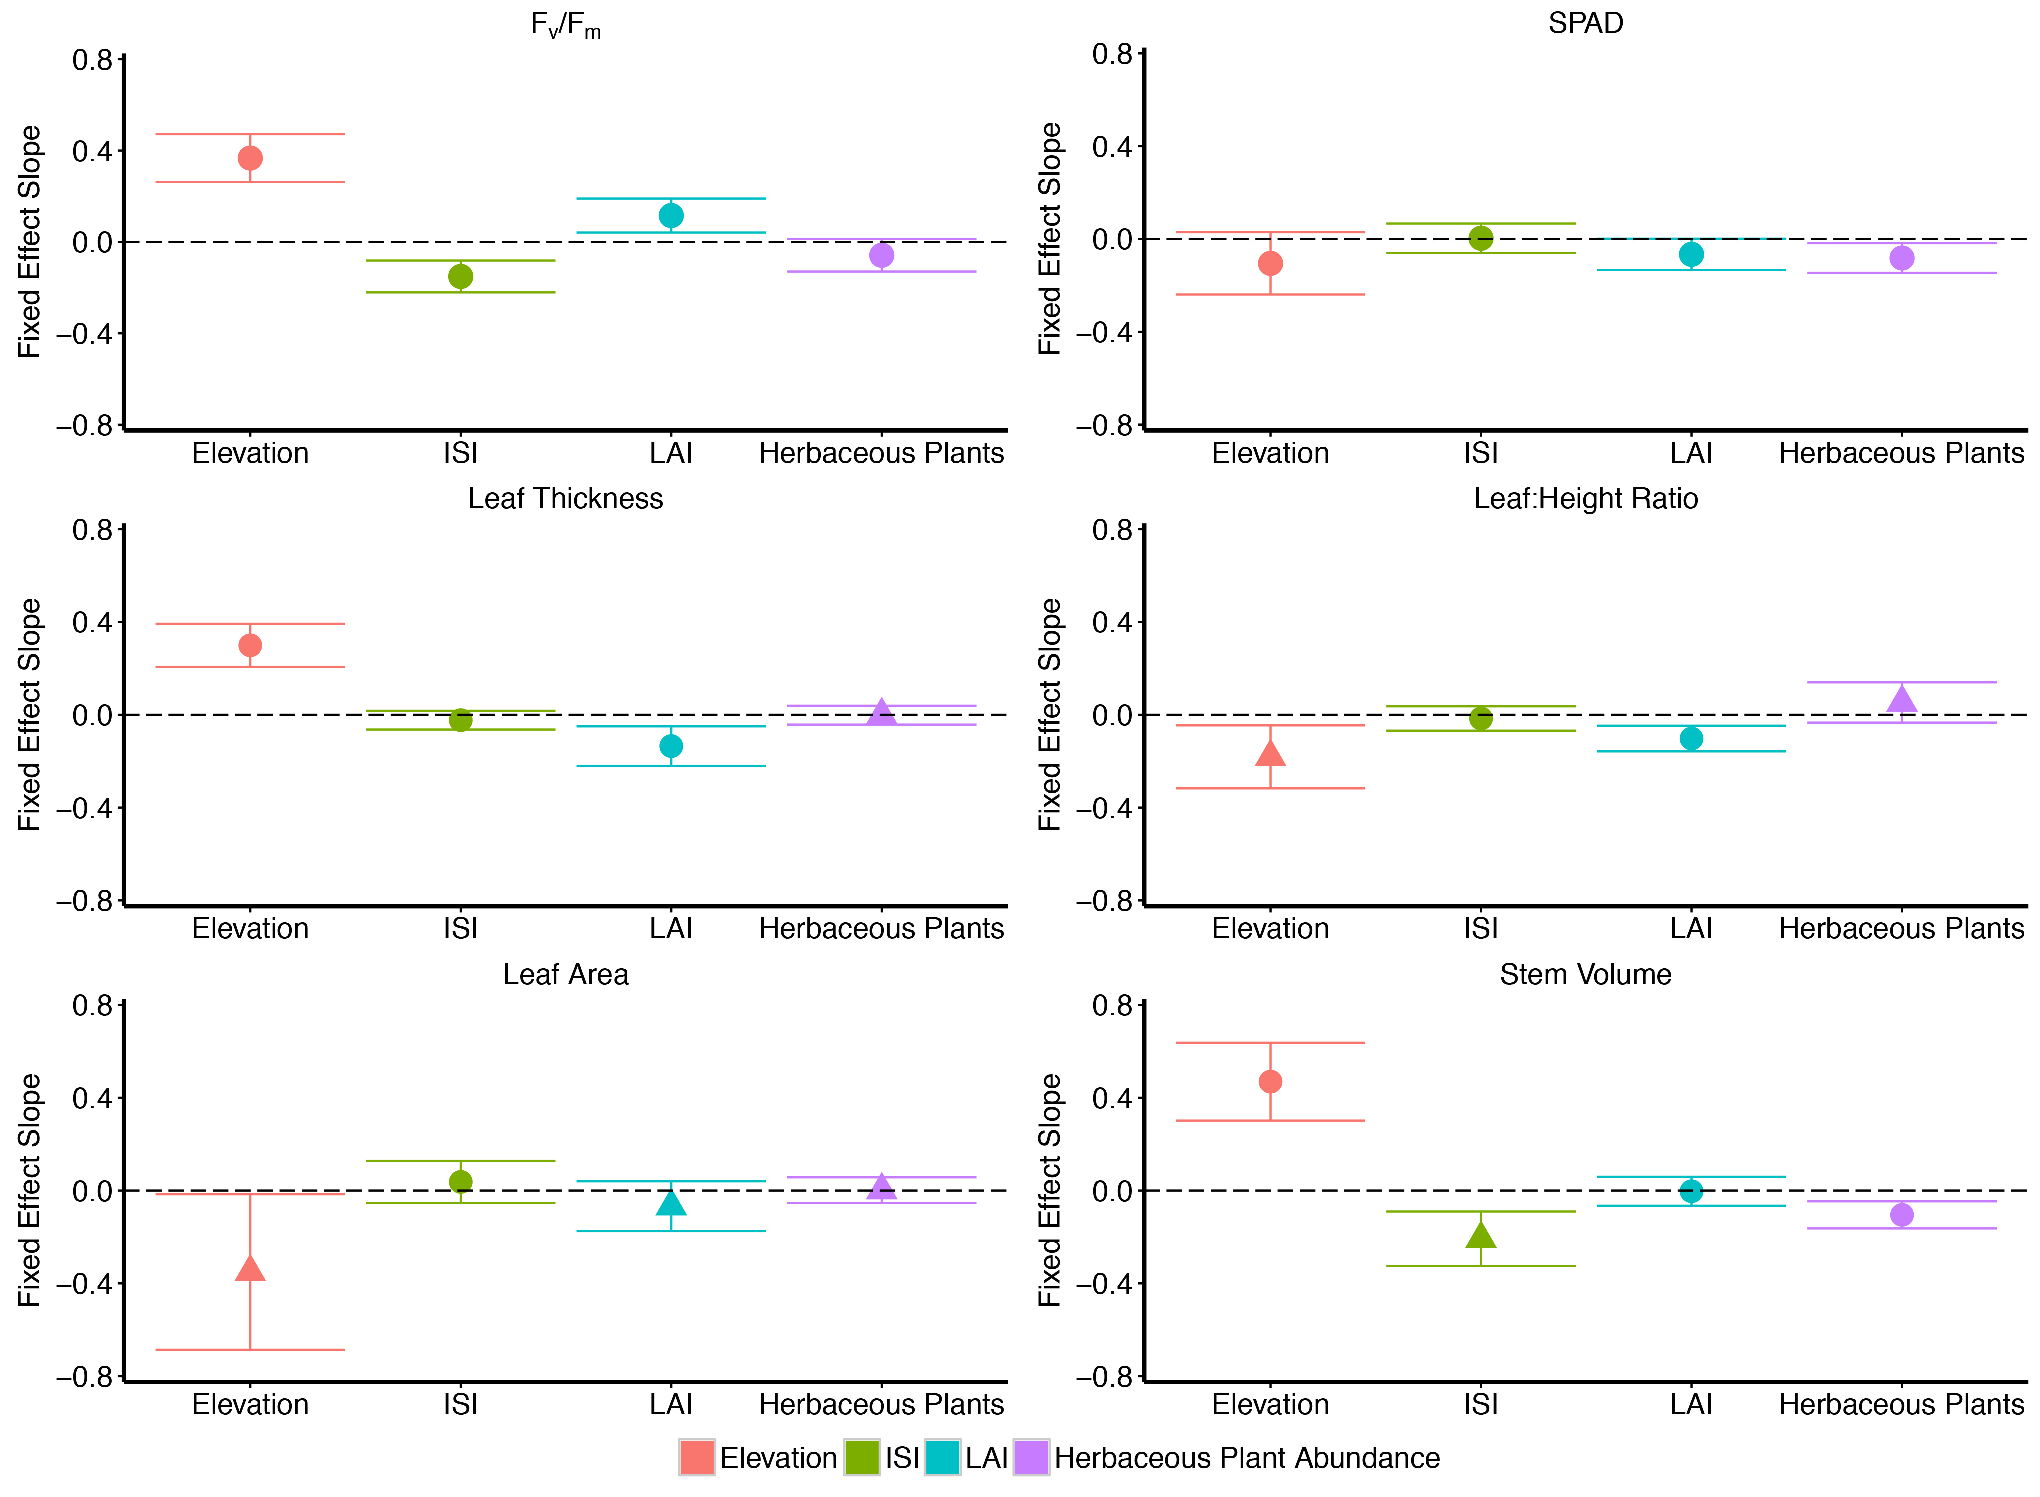
\includegraphics[width = \textwidth]{slope_traits.pdf}
\caption{Fixed effect slopes (points) and standard errors (error bars) for each single fixed effect model. Each panel represents all the models for one plant trait. Model slopes for models where species' slopes were allowed to vary by slope are triangles while those models only allowing species intercept variation are circles. Fixed effects and response variables were standardised to allow easier comparison of effect sizes. Points and error bars are shaded according to the fixed effect used in the model.}
\label{fig:slope_traits}
\end{figure}

\subsection*{Comparison of multiple fixed effect models (H\textsubscript{n2})}
Table \ref{tab:best_fit_multi} shows the fixed effects and model fit measures from the best fitting multiple fixed effect models used to predict plant traits. For plant traits where one or more of the single fixed effect models was better when using a random slope (Figure \ref{fig:traits_dAIC}), the species slopes were allowed to vary for those fixed effects (Table \ref{tab:best_fit_multi} - [\cmark]) in some model iterations. 

All of the best models except the one predicting SPAD included elevation as a fixed effect alongside competition variables. All of the best models were better than a model using only elevation (Appendix IV). The best models for leaf:height ratio, leaf area and stem volume used random slopes for all the fixed effects identified as varying among species in the single predictor models. The fixed effects in the multiple fixed effect models still accounted for a small percentage of the variation in plant traits, ranging from 0.4\% (SPAD), to 17.3\% (stem volume).

When multiple fixed effects were used in a model, the standard errors surrounding the slopes of those fixed effects were reduced (Figure \ref{fig:fix_eff}, Appendix II). The effect of herbaceous plant abundance became larger in the multiple fixed effects model compared to the single fixed effect model. The best LMM for SPAD was no better than a random effects model ($\Delta$AIC\textsubscript{r} = -1.0) and was 14.2\% likely to be better than the next best model, which included only elevation ($W_i$ = 0.142).

% Table created by stargazer v.5.2 by Marek Hlavac, Harvard University. E-mail: hlavac at fas.harvard.edu
% Date and time: Tue, Apr 12, 2016 - 19:54:11
\begin{table}[H] \centering 
  \caption{The form of the best fitting multi-fixed effect model for each plant trait, showing the fixed effects used and various measures of model quality. [\cmark] indicates that a random slope term was included for this fixed effect.}
  \label{tab:best_fit_multi} 
\begin{tabular}{@{\extracolsep{0pt}} ccccccSSSS} 
\\[-1.8ex]\hline 
\hline \\[-1.8ex] 
 & Plant Trait & Elevation & ISI & LAI & Herbaceous  & {$\Delta$AIC\textsubscript{r}} & {$W_i$} & {$R_C^2$} & {$R_M^2$} \\ 
 &&&&&{plants}&&&&\\
\hline \\[-1.8ex] 
& F\textsubscript{v}/F\textsubscript{m} & \cmark & \cmark & \cmark & \xmark & 8.8 & 0.421 & 0.320 & 0.140 \\ 
& SPAD & \xmark &\xmark  & \cmark &\xmark  & -1.0 & 0.142 & 0.325 & 0.004 \\ 
& Leaf Thickness & \cmark & \cmark & \cmark &  \xmark & 12.4 & 0.365 & 0.761 & 0.120 \\ 
& Leaf:Height Ratio & [\cmark] &\cmark  &  \cmark& [\cmark] & 10.7 & 0.620& 0.578 & 0.064 \\ 
& Leaf Area &[\cmark] &\cmark  & [\cmark] &[\cmark]  & 5.8 & 0.296 & 0.801 & 0.071\\ 
& Stem Volume & \cmark &[\cmark]  &\cmark  &\cmark  & 32.3 & 0.610 &0.575 & 0.173 \\ 
\hline \\[-1.8ex] 
\hline \\
\end{tabular} 
\end{table} 

\begin{figure}[H]
\centering
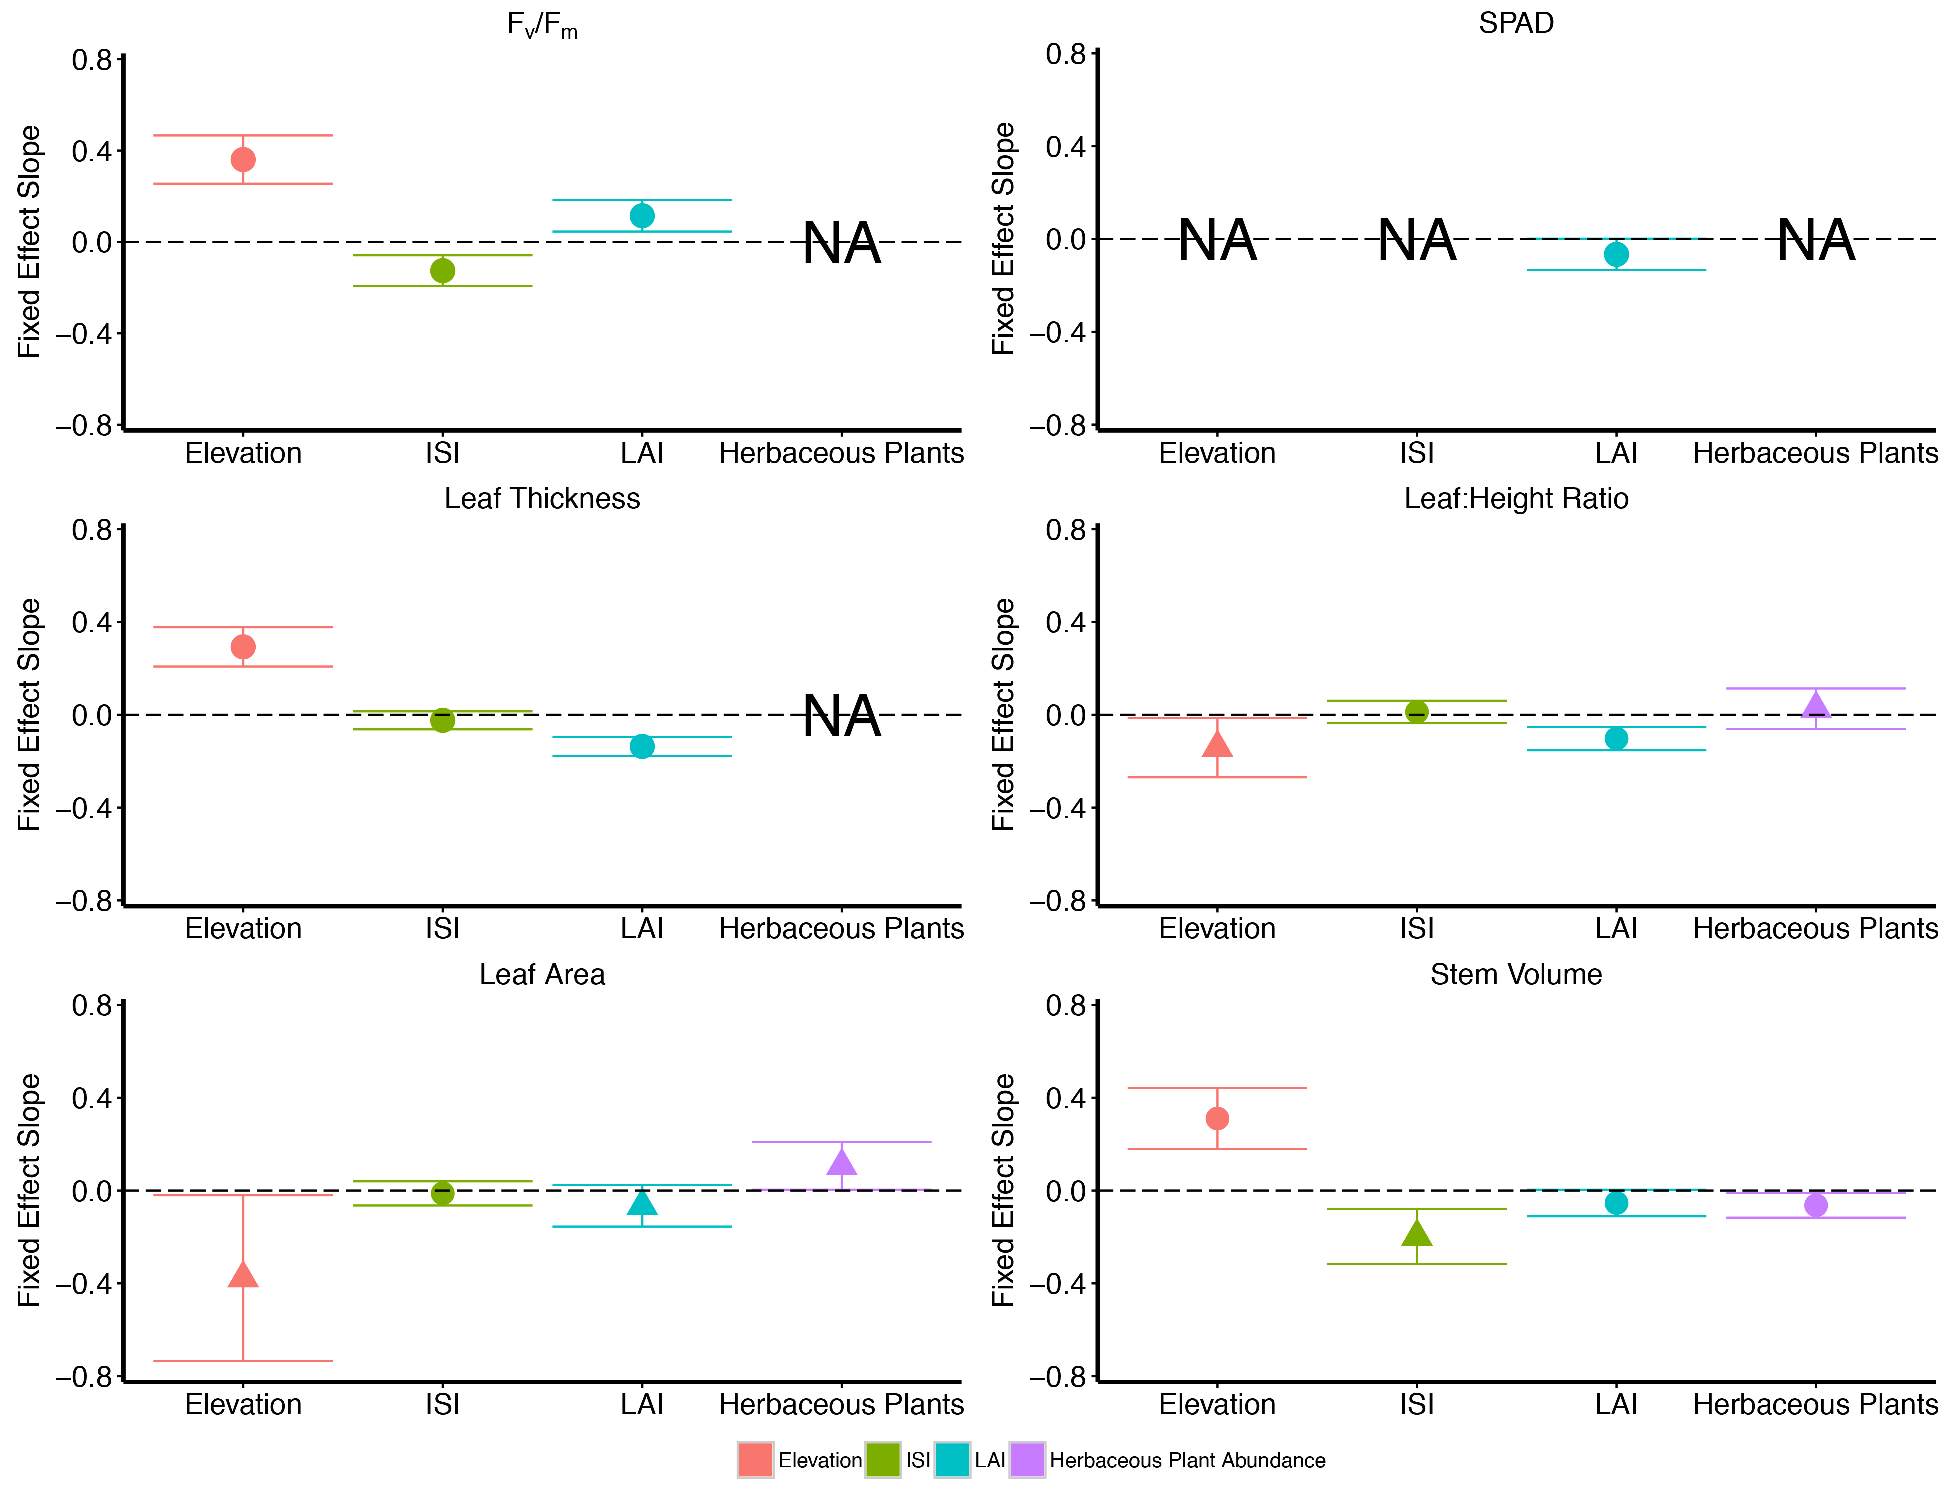
\includegraphics[width = \textwidth]{fix_eff.pdf}
\caption{Fixed effect slopes (points) and standard errors (error bars) for the best multiple predictor models for each plant trait. Predictor variables were all standardised to allow easier comparison of effect sizes. Each panel shows the fixed effect slopes for each fixed effect used in the best model for a given plant trait. Points and error bars are shaded according to the fixed effect used in the model. ``NA" indicates that the given fixed effect was not included in the best model.}
\label{fig:fix_eff}
\end{figure}



%-------------------------------------------------------------------------------------------------------------------
\section{Variation in competition variables across elevation (H\textsubscript{n3})}
\begin{figure}[H]
\centering
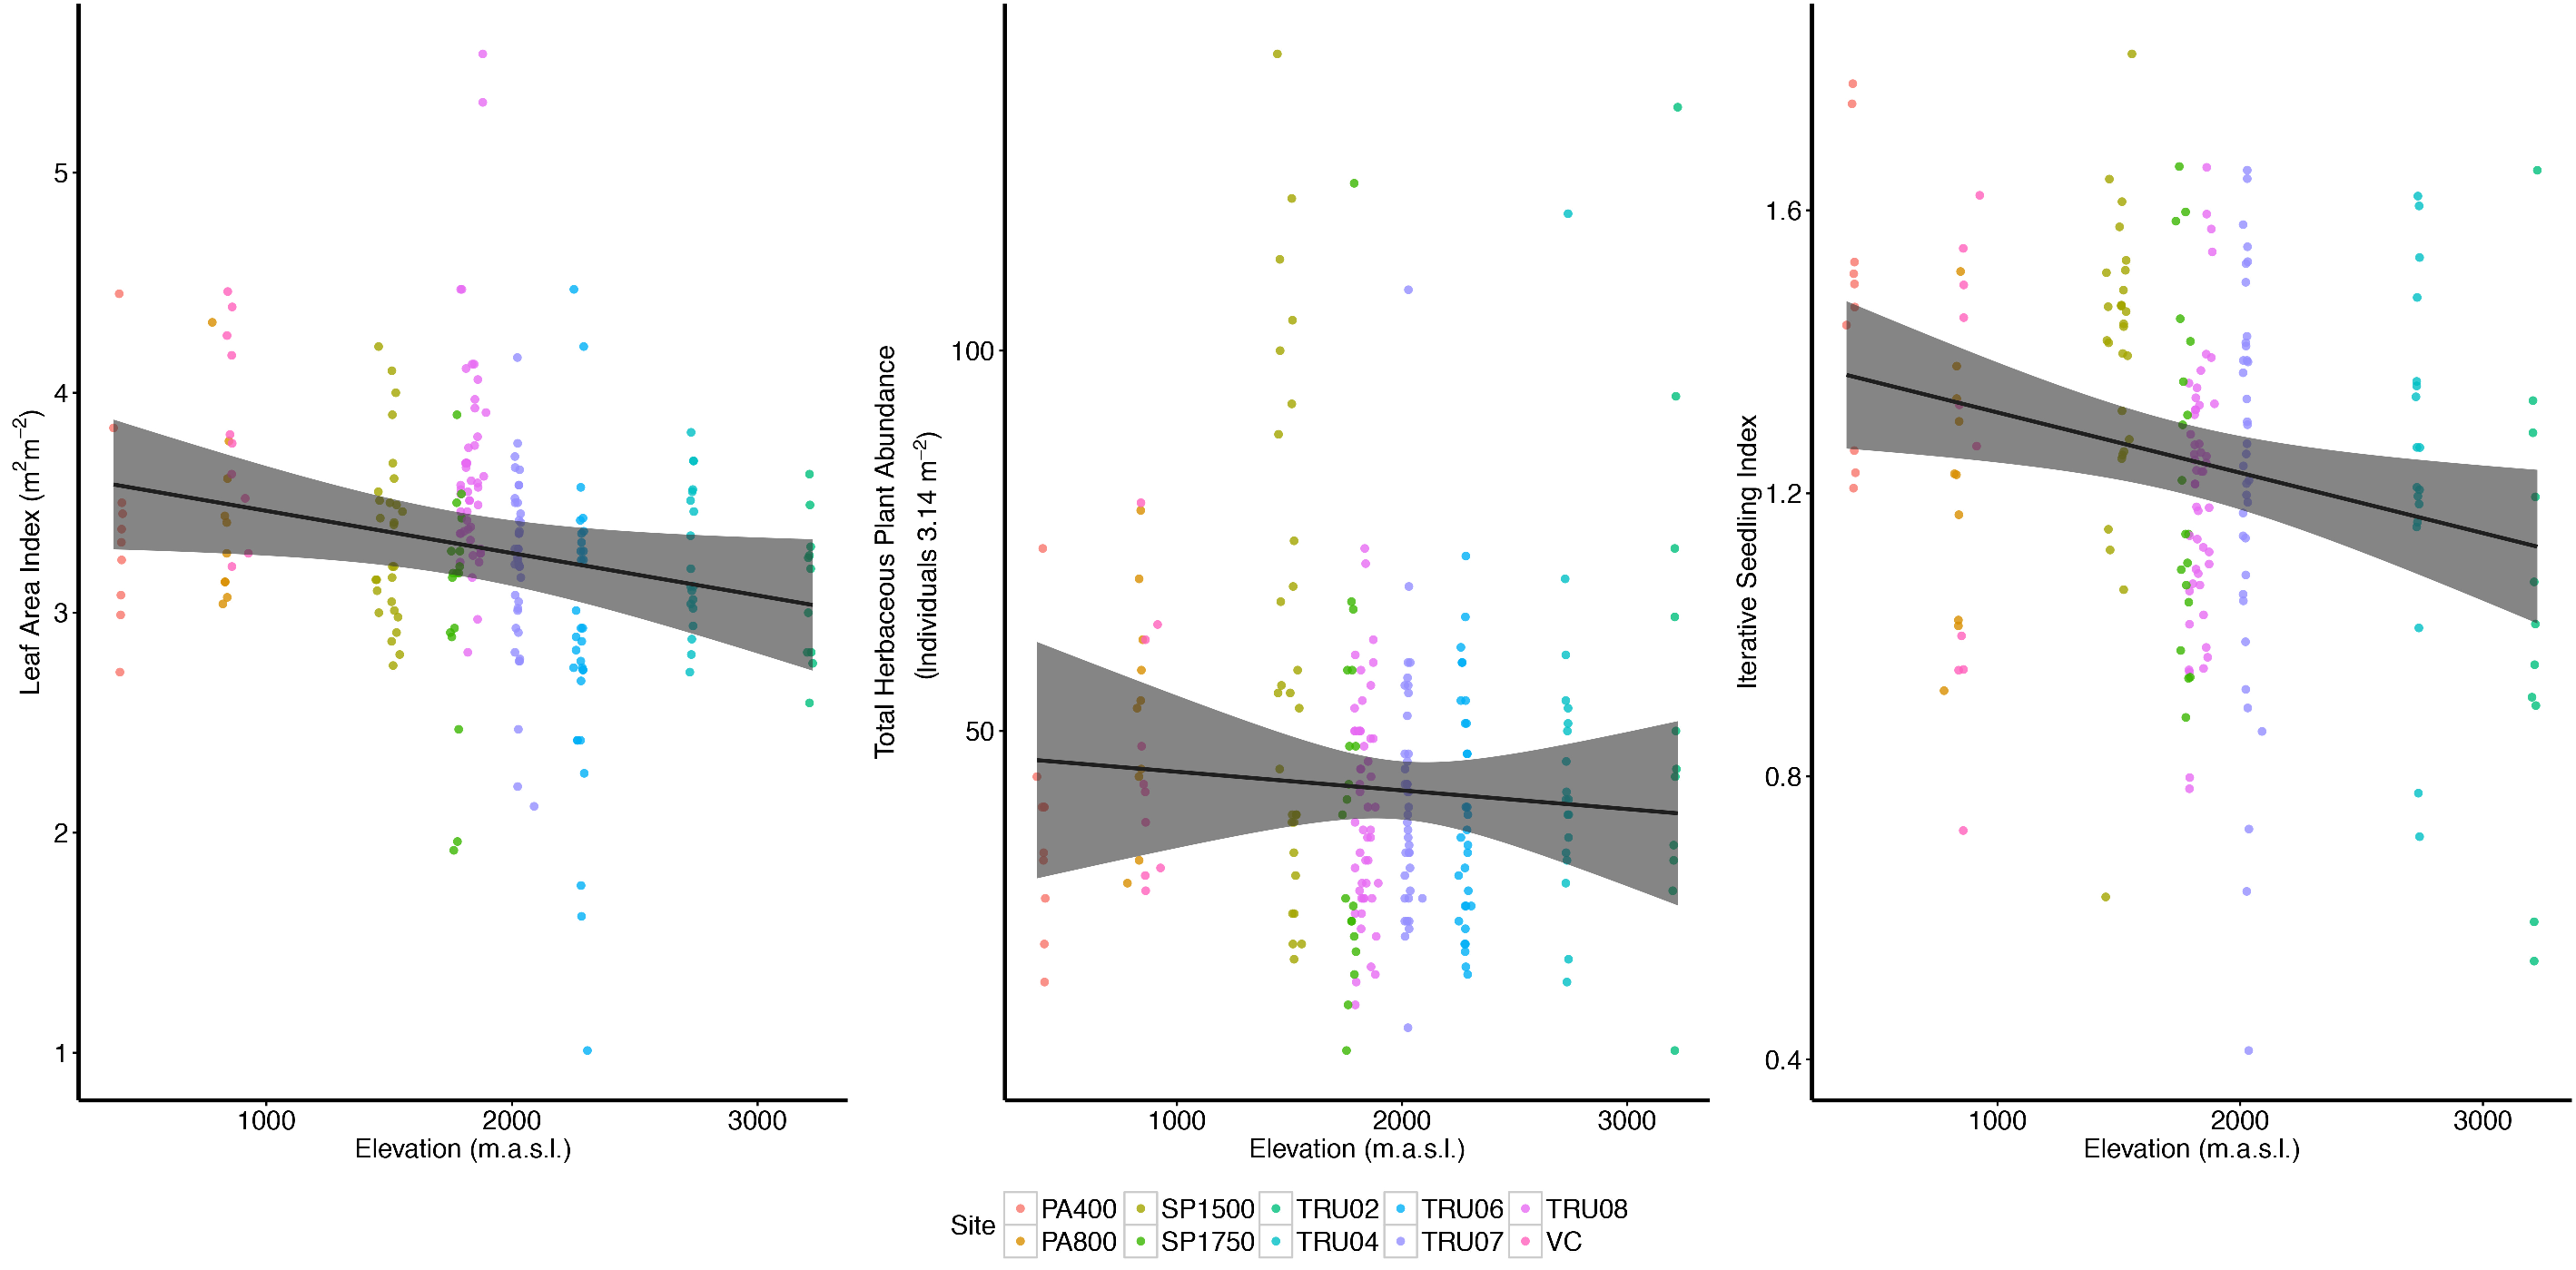
\includegraphics[scale=0.34]{env_elev.pdf}
\caption{Linear mixed model regressions showing how each of the three competition variables vary with elevation. The black line and shaded ribbon show the regression fit and 95\% confidence intervals, respectively. Points are shaded according to site, which was added as a random intercept term.}
\label{fig:env_elev}
\end{figure}

LMMs were conducted for each of the three competition variables (Figure \ref{fig:env_elev}, Table \ref{tab:comp_elev}), giving each site a random intercept. The AIC of each model was compared to a random effects model to assess the explanatory power of elevation. Only ISI varied clearly with elevation, (slope = -8.44 x10\textsuperscript{-5}, SE = 3.661 x10\textsuperscript{-5}, $\Delta$AIC\textsubscript{r} = 8.0), though elevation explained 4.8\% of the variation in ISI. Total herbaceous plant abundance did not vary with elevation, with a random effects model being better than the mixed model ($\Delta$AIC\textsubscript{r} = -4.3). LAI decreased with elevation (slope = -1.92 x10\textsuperscript{-4}, SE = 9.121 x10\textsuperscript{-5}, $\Delta$AIC\textsubscript{r} = 1.8), but this variation may have been due to site level differences ($\Delta$AIC\textsubscript{r}<2). Elevation explained 5.1\% of the variance in LAI. None of the competition variables showed a clear trend with elevation, with large within site variation in all sites (Figure \ref{fig:env_elev}).


% Table created by stargazer v.5.2 by Marek Hlavac, Harvard University. E-mail: hlavac at fas.harvard.edu
% Date and time: Fri, Apr 22, 2016 - 15:46:29
\begin{table}[H] \centering 
  \caption{Model output for three mixed models explaining how competition variables vary with elevation.} 
  \label{tab:comp_elev} 
\begin{tabular}{@{\extracolsep{5pt}}lSSS} 
\\[-1.8ex]\hline 
\hline \\[-1.8ex] 
 & \multicolumn{3}{c}{\textit{Response variable:}} \\ 
\cline{2-4} 
\\[-1.8ex] & {Leaf Area Index} & {Total Herbaceous Plant}  & {Iterative}  \\ 
 & {(m\textsuperscript{2} m\textsuperscript{-2})} &  {Abundance (3.14 m\textsuperscript{-2})} & {Seedling Index} \\
\hline \\[-1.8ex] 
 Elevation & -0.0002 & -0.00005 & -0.0001\\ 
  & (0.0001) & (0.0001) & (0.00003) \\ 
  & & & \\ 
 Constant & 3.656 & 3.835 & 1.400 \\ 
  & (0.178) & (0.276) & (0.063) \\ 
  & & & \\ 
\hline \\[-1.8ex] 
Observations & 
225 & 227 & 193\\ 
$\Delta$AIC\textsubscript{r} & 1.8 & -4.3 & 8.0\\
$R_C^2$ & 0.189 & {NA} & 0.087\\
$R_M^2$ & 0.051 & {NA}& 0.048 \\
\hline \\[-1.8ex] 
Model Type & {LMM} & {GLMM} & {LMM}\\
Family & {Gaussian} & {Negative Binomial}  & {Gaussian}\\

\hline 
\hline \\[-1.8ex] 
\end{tabular} 
\end{table} 

%-----------------------------------------------------------------------------------------
\section{Variation in abiotic environmental variables across elevation}

LMMs including site as a random intercept term were conducted to ascertain soil temperature and moisture varied across elevation. Soil temperature decreased with elevation (slope = 4 x10\textsuperscript{-3}, SE = 4 x10\textsuperscript{-4}, $R^2_C$ = 0.953, $\Delta$AIC\textsubscript{r} = 11.6) (Figure \ref{fig:temp_mois_fit}a). Soil temperature was poorly predicted at extreme high and low elevations. Soil moisture did not vary appreciably with elevation, with a random effects model explaining the variation more parsimoniously (slope = 3 x10\textsuperscript{-3}, SE = 3 x10\textsuperscript{-3}, $R^2_C$ = 0.414, $\Delta$AIC\textsubscript{r} = -1203.985). The fixed effect of elevation accounted for 2.2\% of the variance in soil moisture. 

\begin{figure}[H]
\centering
\includegraphics[scale=0.5]{temp_mois_fit.pdf}
\caption{Linear mixed models showing the variation in soil temperature \textbf{(a)} and soil moisture \textbf{(b)} across elevation. Points are shaded according to site. The thick black line and shaded ribbon show the regression fit and 95\% confidence intervals, respectively. Soil temperature shows a clear decrease with elevation, while soil moisture features high variability within sites.}
\label{fig:temp_mois_fit}
\end{figure}

%-------------------------------------------------------------------------------------------------------------------
\section{Variation in plant traits across elevation (H\textsubscript{n4}, H\textsubscript{n5})}

LMMs allowing each species to vary in slope allowed variation among species to be identified from the model output. Across species, only leaf thickness was better explained by a model including elevation than a model including only the random effects of site and species (Table \ref{tab:plant_traits}). All other plant traits had no clear relationship with elevation ($\Delta$AIC\textsubscript{r} < 2).

\begin{figure}[H]
\centering
\includegraphics[width = 0.674\textwidth]{slope_traits_p1.pdf}
\end{figure}
\vspace{-1cm}
\begin{figure}[H]
\centering
\includegraphics[width=0.674\textwidth]{slope_traits_p2.pdf}
\caption{Scatterplots with linear regressions show the slopes for each species (lines) with 95\% confidence interval (ribbon) with individual seedling measurements (points). Interval plots show the variation in slopes among species for each plant trait (points) with standard errors (error bars).}
\label{fig:trait_elev}
\end{figure}

% Table created by stargazer v.5.2 by Marek Hlavac, Harvard University. E-mail: hlavac at fas.harvard.edu
% Date and time: Tue, Apr 19, 2016 - 17:28:40
\begin{table}[H] \centering 
\begin{adjustwidth}{-0.8cm}{-0.5cm}
\begin{center}
  \caption{Model output for six mixed models explaining how plant traits vary with elevation.} 
  \label{tab:plant_traits} 
\begin{tabular}{@{\extracolsep{-2pt}}l@{\hspace{-10pt}}SSSSSS} 
\\[-1.8ex]\hline 
\hline \\[-1.8ex] 
 & \multicolumn{6}{c}{\textit{Response variable:}} \\ 
\cline{2-7} 
\\[-1.8ex] & {F\textsubscript{v}/F\textsubscript{m}} & {SPAD} & {Leaf}  & {Leaf:height} & {log(leaf area)} & {Stem}\\ 
\\[-1.8ex] &  &  & {thickness (mm)}  & {ratio (leaves cm\textsuperscript{-1})}  & & {volume (cm\textsuperscript{3})} \\ 
\hline \\[-1.8ex] 
 Elevation & 0.00003 & -0.002 & 0.0001 & -0.0001 & 0.0001 & 0.004 \\ 
  & (0.00001) & (0.003) & (0.00002) & (0.0001) & (0.0002) & (0.002) \\ 
  & & & & & & \\ 
 Constant & 0.714 & 41.473 & 0.132 & 0.487 & 2.827 & -4.020 \\ 
  & (0.024) & (5.965) & (0.053) & (0.131) & (0.358) & (3.970) \\ 
  & & & & & & \\ 
\hline \\[-1.8ex] 
Observations & 225 & 223 & 223 & 227 & 220 & 227 \\ 
$\Delta$AIC\textsubscript{r} & 1.61& -8.67&6.03 &-10.97 & -6.35 & 0.42 \\
 $R_M^2$  &  0.075  &  0.022  &  0.068  &  0.011  &  0.001  &  0.156  \\ 
 $R_C^2$  &  0.379  &  0.530  &  0.746  &  0.476  &  0.553  &  0.611  \\ 
\hline 
\hline \\[-1.8ex] 
\end{tabular} 
\end{center}
\end{adjustwidth}
\end{table} 

F\textsubscript{v}/F\textsubscript{m} increased with elevation (Figure \ref{fig:trait_elev}). All species had a positive relationship with elevation except \textit{Myrcia} spp., and \textit{C. revoluta} which did not vary over elevation. Although the overall effect of elevation of F\textsubscript{v}/F\textsubscript{m} was positive, there was a high standard error in this estimate, indicating a low likelihood that there is any consistent variation in F\textsubscript{v}/F\textsubscript{m} across elevation. \textit{A. verticillata} had the steepest positive trend which bore a large standard error. Elevation explained 7.5\% of the variation in F\textsubscript{v}/F\textsubscript{m}, while the random effects of species and site accounted for 30.4\%. \textit{C. revoluta} had the greatest number of individuals with F\textsubscript{v}/F\textsubscript{m} values below the arbitrary 0.7 threshold indicating plant stress \citep{Maxwell2000}, though the number of individuals falling below this threshold did change not markedly across elevation.

SPAD had greatly differing slopes among species, \textit{A. verticillata}, \textit{C. thurifera}, \textit{D. lamarckianum}, \textit{Myrcia} spp., \textit{S. patula} and \textit{T. guianensis} had negative slopes, \textit{I. deltoidea} had a slope near 0, \textit{H. goudotianum} and \textit{C. revoluta}, had positive slopes (Figure \ref{fig:trait_elev}). Elevation accounted for only 2.2\% of the variation in SPAD, while the random effects of site and species account for 50.8\% (Table \ref{tab:plant_traits}).

Leaf thickness increased with elevation. \textit{I. deltoidea}  had a negative slope, \textit{S. patula} did not vary, all other species had similar positive slopes. \textit{A. verticillata} and \textit{C. thurifera} had the greatest variance in leaf thickness, with a leaf thickness ranges of 0.8 mm and 0.4 mm respectively. 

Leaf:height ratio appeared to decrease with elevation, but this estimate has a large standard error, indicating that there may be no real relationship. Species varied in slope direction, \textit{Myrcia} spp., \textit{D. lamarckianum} and \textit{T. guianensis} decreased, \textit{S. patula}, textit{A. verticillata} and \textit{C. thurifera} increased, all other species showed no clear change with elevation.

Variation in leaf area across elevation was best explained when log transformed, a non-log transformed model failed to converge. Leaf area appeared to decrease over elevation but species varied in the direction of their slopes. \textit{A. verticillata}, \textit{I. deltoidea}, \textit{H. goudotianum}, and \textit{T. guianensis} increased with elevation, while \textit{S. patula}, \textit{D. lamarckianum}, and \textit{C. thurifera} decreased with elevation. \textit{Myrcia} spp. and \textit{C. revoluta} varied little. Elevation explained 0.1\% of the variation in leaf area.

Stem volume appeared to  increase with elevation, but this relationship is largely dominated by the influence of \textit{H. goudotianum}, which features some particularly high stem volumes in its upper plot. \textit{I. deltoidea}, \textit{Myrcia} spp., \textit{A. verticillata}, \textit{T. guianensis} and \textit{C. revoluta} show little variation in their stem volume, while \textit{H. goudotianum}, \textit{S. patula}, \textit{C. thurifera} and \textit{D. lamarckianum} show great variation, with a long tail of high values in most plots. \textit{H. goudotianum} is the only species which increases over elevation, \textit{S. patula} and \textit{C. thurifera} decrease, while all other species show little variation across elevation.



%-------------------------------------------------------------------------------------------------------------------
%-------------------------------------------------------------------------------------------------------------------
\chapter{Discussion}
This study aimed to (a) determine whether plant traits were affected by competition variables, (b) assess how the effects of competition compared to that of elevation, and (c) assess the degree to which plant trait-elevation relationships vary among species. It was found that competition variables never influence a given plant trait more than elevation. Adult-seedling competition effects (LAI and ISI) affect plant traits more than seedling-seedling competition (herbaceous plant abundance). LAI and ISI have contrasting effects on plant traits. 

\section{Effect of competition and elevation on plant traits}
Single fixed effect models demonstrated that the three competition variables influence some plant traits ($\Delta$AIC\textsubscript{r} >2, Figure \ref{fig:daic_r2c_traits}a). The effect size of individual competition variables however, did not exceed that of elevation for any plant traits (Figure \ref{fig:daic_r2c_traits}b, Figure \ref{fig:slope_traits}).  The three competition variables, which represent different types of competition, vary in their effects on seedling traits.
\subsection*{Leaf physiology}
Together, SPAD and F\textsubscript{v}/F\textsubscript{m} are useful measures of a plant's health and the integrity of its photosynthetic apparatus \citep{Clark2000}. SPAD is used as a proxy for leaf chlorophyll content \citep{Richardson2002}, while F\textsubscript{v}/F\textsubscript{m} measures the efficiency with which a leaf can utilise light for photosynthesis \citep{Maxwell2000}. This study found contrasting effects of elevation on SPAD and F\textsubscript{v}/F\textsubscript{m}. As elevation increased, photosynthetic efficiency increased but chlorophyll content decreased slightly (Figure \ref{fig:slope_traits}). There is however, large variation in SPAD within sites and elevation explains little of the variance in SPAD (Figure \ref{fig:trait_elev}), meaning this relationship may be erroneous. Competition variables explained comparatively little variation in F\textsubscript{v}/F\textsubscript{m} or SPAD compared to morphological leaf traits (Figure \ref{fig:trait_elev}b).

\subsubsection*{Photosynthetic efficiency}
Single fixed effect models showed that an increase in canopy density (LAI) caused an increase in photosynthetic efficiency (F\textsubscript{v}/F\textsubscript{m}) (Figure \ref{fig:slope_traits}). Specifically, an increase in photosynthetic efficiency under denser canopy may be the result of a more temporally constant microclimate \citep{Amissah2015}. A denser canopy regulates diurnal temperature oscillations by more effectively trapping warm air between the canopy and the forest floor, reducing temperature stress on the plant \citep{Larcher2003}. Increased shading under denser canopy also reduces the potential for seedling desiccation and cavitation, which can cause damage to seedling leaves. As Sun-flecks move across the forest floor they result in rapid leaf temperature increase \citep{Rozendaal2006, Poorter2010}. Additionally, a reduction in direct sunlight reduces the potential for UV-B damage to photosynthetic apparatus \citep{Dobrikova2013}. Diurnal temperature oscillations are generally of greater range at higher elevations \citep{Seidel2005} as is the UV-B insolation fraction \citep{Piazena1996}, suggesting that the beneficial effects of increased canopy density on photosynthetic efficiency may become greater at higher elevations. In this region however, persistent cloud cover at higher elevations throughout the day may result in no increase in incident UV-B, the majority being absorbed by cloud condensation nuclei before it reaches the leaf \citep{Flint2003}.

Canopy density decreases with elevation (Figure \ref{fig:env_elev}), though this trend may be the result of wide within site variance ($\Delta$AIC\textsubscript{r} < 2). This trend concurs with more conclusive results from other studies which show a clear decrease in canopy density with elevation \citep{Kitayama2002, Moser2008}. The more variable relationship seen in this study may be the result of bias in the sampling strategy. LAI was not measured systematically across each site, instead being measured above each sampled seedling. It is expected that seedlings will grow successfully only under canopy where the average light intensity falls between a minimum needed for growth and a maximum that ensures temperature and UV-B stress does not cause the seedling to perish. In this study therefore, extreme canopy densities were probably not sampled. The presence of bias in our sampling strategy is supported by comparing the range of LAI measurements in other studies. For example, \citet{Asner2003}, in a review of 61 tropical evergreen forests, found that LAI ranged from 1.5 to 8. (after outlier exclusion), whereas our LAI estimate ranged from only 1.0 to 5.5, implying that a representative LAI sample was not achieved within each plot.

It is expected that a decrease in canopy density with elevation will lead to more individuals showing signs of stress at higher elevations, due to the factors discussed above. An increase in plant stress limits overall fitness as energy is allocated more to acclimation processes than to fecundity \citep{Reu2011}. This may hinder further upward migration, especially in species with limited dispersal distance such as \textit{I. deltoidea} which relies on seed dispersal by large mammals (predominantly primates) \citep{Russo2005, Kuprewicz2013} over short distances. In this instance however, there is no clear decrease in F\textsubscript{v}/F\textsubscript{m} with elevation within any species ($\Delta$AIC\textsubscript{r} = 1.61), with 8/9 species show an increase in F\textsubscript{v}/F\textsubscript{m} with elevation (Figure \ref{fig:trait_elev}). This suggests that the effect of canopy density in decreasing photosynthetic efficiency across elevation is masked by other environmental variables.

%It must be noted that while there is a positive relationship between photosynthetic efficiency and LAI in this experiment, this does not necessarily equate to an overall increase in photosynthetic rate. As LAI increases, PAR decreases, meaning that at some point, the beneficial effects of canopy cover will be masked by the detrimental effects of shading, leading to a net reduction in biomass accumulation for the seedling and a concurrent decrease in fitness (REF).

In contrast to the effects of LAI, ISI caused a decrease in photosynthetic efficiency. This suggests that the mechanisms by which LAI may affect photosynthetic efficiency (shading, temperature regulation) differ from those of ISI (nutrient competition, water competition, predation mutualisms) \citep{Lewis2000}. Other studies have shown a nutrient competition effect between adult trees and nearby seedlings. \citet{Palik1997} demonstrated that adult trees of greater basal area (equivalent to DBH) cause a larger reduction in soil available nitrogen which subsequently decreased the growth of pine seedlings. Similarly, \citet{Barberis2005} showed that trenching around neotropical tree seedlings in order to decrease root competition increased the growth and leaf nutrient content of the seedlings. In this set of plots, soil moisture is rarely a limiting factor, and insect predators are much rarer in cloud forests than lowland forests \citep{Rodriguez-Castaeda2010}. This suggests that any negative effect of increased ISI on photosynthetic efficiency would be the result of nutrient competition by adult trees.

ISI decreases with elevation (Figure \ref{fig:env_elev}) and a decrease in ISI causes an increase in photosynthetic efficiency. The increase in F\textsubscript{v}/F\textsubscript{m} with elevation may therefore be partly the result of decreased adult-seedling nutrient competition at higher elevations. The large effect of elevation however, implies that other unmeasured environmental variables influence this trend more than simply  a decrease in ISI.

Herbaceous plant density had little effect on F\textsubscript{v}/F\textsubscript{m}. In the single predictor models, the slope was the smallest of all the environmental variables and explained the least variance (Figure \ref{fig:daic_r2c_traits}, Figure \ref{fig:slope_traits}). In the multi-predictor models the best fitting model did not include herbaceous plant density (Table \ref{tab:best_fit_multi}). Other studies have shown that size-asymmetric competition with adults has a much greater role in structuring forest ecosystems than seedling-seedling competition, especially in tropical forests where seedlings are relatively scarce compared to adult trees \citep{Moles2004, Powers2004}. \citet{Paine2008} estimated the area around tree seedlings in neotropical forests within which seedlings affect the availability of resources both above- and below-ground to other seedlings, finding that most zones did not overlap at all. This implies that seedling-seedling competition in neotropical forests is insignificant. 

\citet{Maxwell2000} suggest that generally, optimum F\textsubscript{v}/F\textsubscript{m} is \textasciitilde0.83, and that if F\textsubscript{v}/F\textsubscript{m} falls below \textasciitilde0.8, it is indicative of some kind of plant stress. It is important to note however, that this optimum is likely to vary markedly among species and has been criticised as yet another arbitrary threshold for a dynamic phenomenon \citep{Ghouil2003}. As a conservative estimate, here plants are defined as experiencing physiological stress when F\textsubscript{v}/F\textsubscript{m}<0.7. Figure \ref{fig:trait_elev} shows that only a few individuals fall below this threshold, suggesting that few individuals along the elevational gradient are experiencing stress. Only \textit{C. revoluta} features reduced photosynthetic capacity with elevation. \textit{C. revoluta} also has the most individuals below the 0.7 threshold. This could be evidence that \textit{C. revoluta} individuals experience greater stress at increasing elevations, but the relationship shown here is not strong enough to be conclusive, with large variation within each plot that \textit{C. revoluta} seedlings were sampled. Alternatively other species which feature an increase in photosynthetic efficiency may be experiencing stress at lower elevations, giving support for the hypothesis given by \citet{Campbell2007}, in which species ranges contract from the bottom up. Temperature increase is the most likely source of this increased stress at the lower limits of species ranges, though stress induced by antagonistic interactions from previously lower elevation species that have shifted upslope faster is also possible. Herbivores for example are expected to move upslope faster than tree species due to their mobility and shorter life-cycles \citep{Chen2011}.

\subsubsection*{SPAD}
SPAD value was not clearly influenced by any of the measured competition variables, or elevation (Figure \ref{fig:slope_traits}). SPAD varied largely both within and among species, with large standard errors surrounding the estimates of each species (Figure \ref{fig:trait_elev}, Table \ref{tab:plant_traits}). The best fitting multiple fixed effect LMM for SPAD did not include elevation (Figure \ref{tab:best_fit_multi}), though this model was only 14.2\% more likely to be the best model than the next best model and the fixed effect of LAI accounted for only 0.4\% of the variance in SPAD (Figure \ref{tab:best_fit_multi}). 

The lack of meaningful variation in SPAD contrasts other studies that have shown increases in chlorophyll content in response to shading \citep{Brand1997, Rijkers2000, Rozendaal2006, Dai2009, Zervoudakis2012} and soil nitrogen content \citep{Cechin2004}. In this study however, SPAD did not vary with LAI (shading), ISI (soil nutrient availability) or herbaceous plant abundance. 

The species with the smallest ranges show the steepest decrease in SPAD with elevation (Figure \ref{fig:trait_elev}). From this one could suggest that specialists are more sensitive to increases in elevation in terms of their photosynthetic apparatus. Species with small ranges are interpreted as being more specialist in their environmental requirements \citep{Thuiller2005}.

\subsubsection*{Summary}
Most species demonstrated an increase in F\textsubscript{v}/F\textsubscript{m} with elevation, while SPAD showed little meaningful variation in response to elevation. Adult-seedling competition variables had contrasting effects on F\textsubscript{v}/F\textsubscript{m} while seedling-seedling competition had no effect. A decrease in ISI with elevation may have contributed to the observed increase in F\textsubscript{v}/F\textsubscript{m} with elevation though it is possible that this trend is actually a result of increased stress at lower elevations in response to temperature stress or herbivory stress. H\textsubscript{n1} is therefore accepted for SPAD and rejected for F\textsubscript{v}/F\textsubscript{m}. The best multiple fixed effect model for F\textsubscript{v}/F\textsubscript{m} included all competition variables, H\textsubscript{n2} is therefore rejected for F\textsubscript{v}/F\textsubscript{m}. SPAD is predicted equally poorly by elevation and competition variables.
%---------------------------------------------------------------------------------------------------------------------------------------------------%---------------------------------------------------------------------------------------------------------------------------------------------------
\subsection*{Leaf and plant morphology}
Leaf thickness increased with elevation. Other studies have also found positive correlations between leaf thickness and elevation, identifying climatic drivers such as mean daily insolation and diurnal temperature variation \citep{Niinemets2001}, which lead to reduced leaf pay-back times and a need to grow leaves that can survive the more variable environmental conditions found at higher elevations \citep{Milla2011}. Increased UV-B results in an increase in cuticle thickness, to reduce the concentration of UV-B absorbed by photosystem II  (PSII) where it can cause damage and thus photoinhibition \citep{Vass1997, Szilard2007}. In this study however, it is unclear whether the insolation UV-B fraction does increase with elevation as it was not measured. Additionally, it is expected that frequent cloud immersion in the high elevation sites would reduce UV-B absorption and thus the need for thick cuticles. Leaf thickness decreased under increased canopy density (Figure \ref{fig:slope_traits}), adding support to the conclusion that increased direct sunlight is the cause of the decrease in leaf thickness with elevation.

Leaf area variation was explained poorly by both competition variables. Previous studies have shown a clear decrease in leaf area with elevation, citing decreases in canopy density and an increase in nutrient competition with elevation as drivers of this variation \citep{Pan2013}. Plants with access to higher resource levels generally invest in leaves which can achieve a higher photosynthetic rate per energy input in leaf construction, at the expense of leaf longevity \citep{Mediavilla2009}. In the plots studied here however, available nitrogen does not decrease with elevation, though elevational variation in other nutrients is not known.

Leaf:height ratio decreased with elevation (Figure \ref{fig:slope_traits}) meaning that plants became less leafy per unit stem height as elevation increased.  However this relationship explained very little of the variance in leaf:height ratio (Table \ref{tab:plant_traits}). Competition variables had little effect on leaf:height ratio (Figure \ref{fig:slope_traits}). Few studies have focussed specifically on measures of leaf:height ratio or number of leaves as an adaptive/acclimatory trait though we may interpret that a reduction in ``leafiness" is an extension of the trend seen in reduced leaf area with elevation. Seedlings may be more likely to produce fewer leaves in order to allocate more biomass to structural support in those leaves that are grown \citep{Onoda2011}.

Stem volume decreased with ISI (Figure \ref{fig:slope_traits}). This may have contributed to the increase in stem volume with elevation, as ISI decreases with elevation (Figure \ref{fig:env_elev}). Other studies have found that stem volume increases with average wind speed in order to provide greater stem support \citep{Onoda2011}, and that stems become more elongated as diurnal temperature range increases \citep{Myster1995}. Wind speed is expected to increase with elevation as is diurnal temperature range, providing further support for the trend seen here. An increase in stem volume with elevation suggests that tree seedlings are allocating less biomass to other parts such as the leaves, meaning that plant growth may be slower at higher elevations. This is supported by the negative relationship between leaf area and elevation, and the negative relationship between leaf:height ratio and elevation, which suggests that seedlings produce fewer, smaller leaves as elevation increases.

\subsection*{Summary}
Stem volume was the only morphological plant trait that showed clear variation with a competition variable (ISI), therefore H\textsubscript{n1} is accepted for all other morphological plant traits. All morphological plant traits were best explained by a multiple fixed effect model including elevation and a combination of competition variables, therefore H\textsubscript{n2} is accepted for all morphological plant traits. Morphological plant traits varied across elevation in a manner similar to that identified by previous studies, responding to elevation dependent abiotic environmental variables such as temperature and nutrient availability. The strength of the relationships seen here is not as great as that demonstrated by other studies, possibly because of the comparatively low sample size per species in this study compared to larger reviews and the presence of confounding environmental variables that were not accounted for in statistical analysis.

\section{Variation in plant traits with elevation}
Within each species, plant traits vary across elevation, with slope standard errors overlapping zero in only a few instances (Figure \ref{fig:trait_elev}). H\textsubscript{n4} can therefore be rejected, and it can be concluded that the individuals sampled in this study are acclimating their morphology in response to elevationally dependent environmental variables. The difference in magnitude and direction of the relationships shows that species are responding differently to changes in elevation. Supporting the observations and predictions of other studies that species are likely to migrate at different rates to climate change. Those species showing increased morphological change with elevation are expected to be more sensitive to changes in climate and are thus more likely to show greater migration rates.

\subsection*{Variation among species}
Species varied largely in the direction, magnitude and variance of their plant trait response to elevation (Figure \ref{fig:trait_elev}), therefore H\textsubscript{n5} is rejected. Variation among species in slope implies that species differ in their sensitivity to changing environmental conditions across elevation. \textit{D. lamarckianum} and \textit{I. deltoidea}, the two monocot species, show no similarity in their plant trait response to elevation, often having different slope directions for a given plant trait. Together, \textit{D. lamarckianum} and \textit{I. deltoidea} show no difference to dicot species in terms of their plant trait-elevation relationship. \textit{A. verticillata} has a comparatively large variance for all trait-elevation relationships except stem volume. This implies that \textit{A. verticillata} is either more sensitive to changes in climate, or that it has a larger acclimatory range than other species; both may be true. \textit{A. verticillata} has a very small elevational range (Figure \ref{fig:range_plot}) but is also one of the most common tree species found along this set of plots (Appendix VI). This supports the theory that common species have a wider acclimatory range and that species with small ranges are sensitive to environmental variation. In contrast, \textit{Myrcia} spp. has little variation in plant traits compared to other species but has the largest elevational range, the \textit{Myrcia} spp. species sampled are among the rarer species sampled.

Leaf thickness had a similar positive relationship with elevation in 7/9 species, whereas \textit{I. deltoidea} and \textit{S. patula} featuring reduced leaf thicknesses with elevation (Figure \ref{fig:trait_elev}). \textit{C. thurifera} had exceptionally high variance compared to other species, this is due to dense and prominent leaf vein structure in this species (Appendix V). For many \textit{C. thurifera} individuals, the diameter of the micrometer used to measure leaf thickness was too wide to be placed between the prominent leaf veins, leading to an over-estimation of leaf thickness for these individuals. Regardless, \textit{C. thurifera} showed a similar increase in leaf thickness with elevation. \textit{I. deltoidea} had the steepest decrease in leaf thickness over elevation (Figure \ref{fig:trait_elev}). This trend may be a peculiarity of the species or a result of environmental conditions at the upper sample plot for this species (VC). It is impossible to confirm whether site level variation at VC had a peculiar effect on \textit{I. deltoidea} leaf thickness as \textit{I. deltoidea} was the only species sampled at this site. Potentially, the greater leaf thickness at PA400 compared to VC is due to an adaptation to increased herbivory pressure at PA400. There is no evidence for this increase in herbivory in lowland plots other than a general trend that herbivory pressure decreases with elevation in tropical forests \citep{Rodriguez-Castaeda2010}.


\subsection*{Summary}
Tree seedlings are responding to changes in elevationally dependent environmental variables by altering their morphology. Additionally, the strength of the plant trait response varies between species, suggesting that some species are more sensitive to environmental change than others. 

The lack of a clear relationship between plant traits and competition intensity, suggests that tree seedlings are not affected by the biotic environment at the extremes of their ranges more than they are by other environmental variation. Species will therefore continue to migrate upslope, largely unimpeded by changes in biotic environment. It is possible that species will encounter biotic environmental thresholds beyond which adaptation and acclimation are no longer able to prevent stress and increased mortality. In order to answer these questions experimental transplantation is recommended, in order to place individuals outside of their current range. Even then, experimental transplantations do not account for potentially rapid micro-evolution that may occur as species migrate into novel environments. Sufficiently rapid micro-evolution could result in species being able to migrate upslope almost indefinitely, as they adapt and become more able to acclimate to changing climates.

\section{Predictions for future species migration}
This study confirms that adult-seedling competition intensity decreases with elevation (H\textsubscript{n3}), and that this decrease causes some proportion of the effect of elevation on plant traits, though this proportion is likely to be small as LMMs show that elevation still has the greatest influence over plant traits, despite including competition variables alongside elevation in multiple fixed effect models. As such, species may continue to move upslope as temperature increases, without being negatively affected physiologically at the upper limits of their ranges by adapting their morphology to the changing environment. The results from this study however, cannot be used to determine what will happen if a species reaches its adaptational limits as its range shifts. Given that few species experienced physiological stress, it is suggested that none of the species sampled have reached this limit yet. The exception being \textit{C. revoluta}, which shows some evidence of increased physiological stress with elevation and relatively flat relationships between elevation and plant traits, though this trend cannot be confirmed without more study.

Most species featured a decrease in photosynthetic efficiency at the bottom of their elevational ranges. This implies that these species may experience progressively greater plant stress at the bottom of their ranges as temperature increases, and the bottom of their range will continue to shift upslope as a result. This study cannot infer whether the contraction of species' lower range limits will be faster or slower than the expansion of the upper range limit, though other studies have suggested that lower range limits will shift upslope faster than upper limits \citep{Campbell2007}, owing to climate change proceeding faster than micro-evolutionary processes to adapt to higher elevations. This will lead to an overall reduction in range size for many species.

\section{Limitations of this study}
This study sampled seedling physiology over a narrow time period. While F\textsubscript{v}/F\textsubscript{m} and SPAD are unlikely to vary on a daily basis, they may do over the course of a season \citep{Porcar-Castell2008}. Seedlings are likely to alter their leaf physiology and morphology in response to a temporally heterogeneous environment throughout the course of their life. As canopy gaps open and close the light and precipitation regime will change. The measured physiological responses of individuals therefore may not be representative of its physiology over a lifetime. Furthermore, this study only measured seedlings, ignoring other life stages. This means the results of this study cannot be used to directly infer the effects of biotic interactions on plant traits across entire populations. It is likely however, that established adult trees will be less sensitive to competition from other adult trees and completely insensitive to competition from seedlings \citep{Paine2008}. 

Nine tree species were selected for this study. Although these species are common in the areas we sampled (Appendix VI), there are many other species which may react more or less to the biotic environment. There is evidence that rare species are more affected by environmental factors \citep{Lyons2005,Mouillot2013}. Rare species are more likely to occupy specialist niches, which are narrower on a local geographical scale than those of generalist species \citep{Boulangeat2012}. The evolutionary histories of specialists means they are less likely to be able to acclimate to novel environments. Compared to the common species studied here, rare species will not have such a large direct effect on globally significant ecosystem services such as carbon sequestration, albedo, and drainage. This does not mean that rare species do not have the potential to heavily influence ecosystem services indirectly. \citet{Lyons2001}, and \citet{Lyons2005} found that less common species play vital supporting roles in maintaining ecosystem functions such as enhancing invasion resistance and making limiting resources available to other species  . 

There is large potential for falsely inferring causation from the results of this study. Along elevational gradients many environmental factors both abiotic and biotic co
vary. For example, this study concluded that an increase in ISI caused a decrease in photosynthetic efficiency. However, it was found that ISI covaries with elevation, along with many other potential unmeasured environmental variables, therefore photosynthetic efficiency may have merely inversely correlated with ISI rather than ISI causing the variation in photosynthetic efficiency, despite well-documented supporting evidence.

This study is deliberately wide in its scope, using competition intensity proxies in order to infer the influences of many ecosystem processes such as nutrient competition, shading, etc.. By not explicitly testing the effects of these mechanistic processes, which are complex in their effects, we cannot determine the relative contribution of each process implicit in each competition proxy. It is recommended therefore that experiments under constant environmental conditions explicitly test the effect of variation in ecosystem processes which are implied to change as a result of variation in the competition proxies measured here, such as nutrient availability and shading.

The study did not use experimental treatments. It could be argued therefore that measured seedlings would have been unlikely to show stress at all, as seedlings would not have grown to the minimum size needed for measurement otherwise.

\section{Further research}
On the basis of this study, which shows that adult-seedling competition intensity varies across elevation and that this variation forms part of the observed plant trait response to elevation, it is recommended that future studies aim to identify competition intensity thresholds beyond which individuals cannot acclimate to the environmental conditions. The location of thresholds should be confirmed using experimental transplantation of seedlings to different elevations to observe variation in plant traits.

In order to determine whether changes in competition intensity also affect adult trees, and thus recruitment, similar studies should be performed on adult trees. This would help to improve the accuracy of species range-shift models by adding the potential variation found within populations and allowing demographically explicit models.

\chapter{Conclusions}
This study has provided an estimation of the relative effects of seedling-seedling and adult-seedling competition on neotropical tree seedling plant traits, thereby evaluating the potential for competition effects to limit vertical range shifts in response to anthropogenically induced temperature increase. This study found that the intensity of adult-seedling competition affected photosynthetic efficiency, stem volume and leaf thickness. Investigation of the variation in these competition proxies over elevation showed that competition effects form part of a complement of environmental variables that covary across elevation, resulting in an overall variation in plant traits with elevation.

Multiple fixed effect models were of better quality when including competition variables alongside elevation as predictors of plant traits. In light of this, it is suggested that adult-seedling competition proxies or more direct measures of adult-seedling competition are included in future species distribution models alongside climatic variables in order to more accurately and precisely predict species migrations.

This study cannot make direct predictions of how species will react to environmental conditions outside of those measured here. Instead it is suggested that future studies focus on experimental transplantation of seedlings to elevations outside of their current ranges in order to build more realistic predictions of future range shift potential. 

There was marked variation between species in their plant trait response to elevation. This provides supporting evidence for conclusions of other studies which either predict or demonstrate that species differ in their sensitivity to variation in environment and will therefore be likely to vary in their rate of upslope migration. The presence of species specific range shift trends supports the conclusion that biotic environmental effects should be included in range-shift models, as they are only likely to become stronger over time as species ranges overlap.



\clearpage
\singlespacing
\bibliography{Dissertation_Ref}

\clearpage
%---------------------------------------------------------------------------------------------------------------------------------------------------------------------------------------------------------------------------------------------------------------------------------------------------------------------------------------------------------------------------------------------------------------------------------------------------------
\chapter{Appendices}

Appendix I: Model comparison of generalised linear mixed models assuming different error distributions, of the relationship between elevation and herbaceous plant abundance. A negative binomial distribution has a higher $\Delta$AIC\textsubscript{r} and was thus chosen as the best model.
\begin{table}[H] \centering 
  \label{} 
\begin{tabular}{@{\extracolsep{0pt}}lS[table-figures-integer = 3]S} 
\\[-1.8ex]\hline 
\hline \\[-1.8ex] 
 & \multicolumn{2}{c}{\textit{Model Type:}} \\ 
\cline{2-3} 
\\[-1.8ex] & {GLMM} & {GLMM} \\ 
\\[-1.8ex] & {Poisson} & {Negative Binomial}\\ 
\hline \\[-1.8ex] 
 Elevation & -0.001 & -0.00005 \\ 
  & (0.001) & (0.0001) \\ 
  & & \\ 
 Constant & 4.898 & 3.835 \\ 
  & (1.173) & (0.276) \\ 
  & & \\ 
\hline \\[-1.8ex] 
Observations & 227 & 227 \\ 
$\Delta$AIC\textsubscript{r} & -287.2  & -4.3 \\ 
\hline 
\hline \\[-1.8ex] 
\end{tabular} 
\end{table} 


Appendix II: Full mixed effects model output for the best multiple fixed effects model explaining each plant trait. `NA' indicates that a fixed effect was not used in the best model.
% Table created by stargazer v.5.2 by Marek Hlavac, Harvard University. E-mail: hlavac at fas.harvard.edu
% Date and time: Sun, Apr 24, 2016 - 19:07:11
\begin{table}[!htbp] \centering 
\begin{adjustwidth}{-0.8cm}{-0.5cm}
\begin{center}
 \label{} 
\begin{tabular}{@{\extracolsep{0pt}}l@{\hspace{-2pt}}SSSSSS} 
\\[-1.8ex]\hline 
\hline \\[-1.8ex] 
 & \multicolumn{6}{c}{\textit{Response variable:}} \\ 
\cline{2-7} 
\\[-1.8ex] & {F\textsubscript{v}/F\textsubscript{m}} & {SPAD} & {Leaf} & {Leaf:height}  & {log(Leaf area)} & {Stem}  \\ 
\\[-1.8ex] &  &  & {Thickness (mm)}  & {ratio (leaves cm\textsuperscript{-1})} & {(mm\textsubscript{2})} & {Volume (cm\textsuperscript{3})}\\ 
\hline \\[-1.8ex] 
\bfseries{Fixed Effects} & & & & & & \\
 LAI & 0.115 & -0.066 & -0.136 & -0.103 & -0.066 & -0.054 \\ 
  & (0.069) & (0.067) & (0.041) & (0.050) & (0.090) & (0.057) \\ 
  & & & & & & \\ 
 Herbaceous  & {NA} & {NA}  & {NA} & 0.026 & 0.106 & -0.064 \\ 
 Plant Abundance & {(NA)} & {(NA)}  & {(NA)}  & (0.087) & (0.103) & (0.053) \\ 
  & & & & & & \\ 
ISI & -0.126 & {NA}  & -0.024 & 0.012 & -0.012 & -0.198 \\ 
  & (0.068) & {(NA)} & (0.039) & (0.048) & (0.052) & (0.119) \\ 
  & & & & & & \\ 
Elevation & 0.361 & {NA}  & 0.293 & -0.141 & -0.377 & 0.310 \\ 
  & (0.106) & {(NA)} & (0.085) & (0.128) & (0.358) & (0.132) \\ 
  & & & & & & \\ 
 Constant & -0.003 & 0.076 & 0.018 & 0.016 & -0.028 & 0.038 \\ 
  & (0.083) & (0.101) & (0.137) & (0.105) & (0.118) & (0.098) \\ 
  & & & & & & \\ 
\hline \\[-1.8ex] 
Observations & 191 & 191 & 191 & 191 & 189 & 191 \\ 
$\Delta$AIC\textsubscript{r} & 8.8 & -1.0 & 12.4 & 10.7 & 5.8 & 32.3 \\ 
$R_C^2$ &0.320 &0.325 &0.761 &0.578 & 0.802 &0.575 \\
$R_M^2$ &0.140 &0.004 &0.120 &0.030 &0.071 &0.173 \\
\hline 
\hline \\[-1.8ex] 
\end{tabular}
\end{center}
\end{adjustwidth} 
\end{table}
\clearpage
Appendix III: Comparison of models allowing species to vary either by intercept or slope ($\Delta$AIC\textsubscript{r} and the comparison of the best of these two models to a random effects model ($\Delta$AIC\textsubscript{r}, Slope, $R_C^2$). Elev. = Elevation, LAI = Leaf Area Index, HPA = Herbaceous Plant Abundance, ISI = Iterative Seedling Index. RS/RI indicates whether a random intercept (RI) or random slope (RS) model was of better quality according to AIC.
% Table created by stargazer v.5.2 by Marek Hlavac, Harvard University. E-mail: hlavac at fas.harvard.edu
% Date and time: Tue, Apr 12, 2016 - 17:11:16
\begin{table}[H] \centering 
  \label{} 
\begin{tabular}{@{\extracolsep{5pt}} ccScSS[table-figures-integer = 4, table-figures-decimal=3]
S} 
\\[-1.8ex]\hline 
\hline \\[-1.8ex] 
 & Fixed Effect & {$\Delta$AIC\textsubscript{rsri}} & {RS/RI} & {$\Delta$AIC\textsubscript{r}} & {Slope} & {$R_C^2$} \\ 
\hline \\[-1.8ex] 
F\textsubscript{v}/F\textsubscript{m} & Elev. &    - 11.8 & RI &    - 13.4 & 0.00003 & 0.287 \\ 
 & LAI &    - 3.4 & RI &    - 7.5 & 0.01 & 0.258 \\ 
 & HPA &    - 2.6 & RI &    - 5.7 &    - 0.0001  &  0.246  \\ 
 & ISI &    - 3.3 & RI &    - 9.6 &    - 0.03  &  0.238  \\ 
\hline \\[-1.8ex] 
SPAD & Elev. &    - 8.8 & RI &    - 43.8 &    - 0.001  &  0.305  \\ 
 & LAI &  1.0 & RS &    - 45.3 &    - 1.40  &  0.355  \\ 
 & HPA &    - 3.2 & RI &    - 44.8 &    - 0.031  &  0.324  \\ 
 & ISI &  1.1 & RS &    - 44.4 &  1.4  &  0.338  \\ 
\hline \\[-1.8ex] 
Leaf Thickness & Elev. &    - 10.0 & RI &    - 207.5 &  0.0001  &  0.750  \\ 
(mm) & LAI &  23.2 & RS &    - 232.5 &    - 0.04  &  0.760  \\ 
 & HPA &    - 3.9 & RI &    - 200.0 &    - 0.00001  &  0.738  \\ 
 & ISI &    - 3.9 & RI &    - 200.3 &    - 0.01  &  0.739  \\ 
\hline \\[-1.8ex] 
Leaf:height ratio & Elev. &    - 9.5 & RI &    - 72.3 &    - 0.001  &  0.416  \\ 
(leaves cm\textsuperscript{-1}) & LAI &    - 2.3 & RI &    - 72.7 &  0.7  &  0.402  \\ 
 & HPA &    - 3.8 & RI &    - 74.4 &    - 0.03  &  0.419  \\ 
 & ISI &    - 1.0 & RS &    - 71.8 &  1.3  &  0.418  \\ 
\hline \\[-1.8ex] 
log(Leaf area) & Elev. &    - 0.3 & RI &    - 86.6 &  0.001  &  0.491  \\ 
(mm\textsuperscript{2}) & LAI &  8.8 & RS &    - 95.4 &    - 8.5  &  0.608  \\ 
 & HPA &  1.0 & RS &    - 87.6 &  0.1  &  0.554  \\ 
 & ISI &  5.1 & RS &    - 91.7 &  9.0  &  0.496  \\ 
\hline \\[-1.8ex] 
Stem volume & Elev. &    - 4.5 & RI &    - 74.3 &  4.3  &  0.537  \\ 
(cm\textsuperscript{3}) & LAI &    - 3.4 & RI &    - 68.1 &    - 35.8  &  0.558  \\ 
 & HPA &    - 2.0 & RI &    - 71.3 &    - 27.9  &  0.575  \\ 
 & ISI &  21.5 & RS &    - 101.5 &    - 4866.6  &  0.560  \\ 
\hline \\[-1.8ex] 
\hline \\
\end{tabular} 
\end{table} 
\clearpage
Appendix IV: Full model comparison of multiple fixed effect models for each plant trait (a - f), ranked by AIC. $\Delta$AIC\textsubscript{r} is the $\Delta$AIC between a random effects model and that model. Models highlighted in \textbf{bold} were chosen as the best model on the basis of $\Delta$AIC\textsubscript{r} $R_C^2$ and $W_i$ and reported in the main text. Elev. = Elevation, ISI = Iterative Seedling Index, LAI = Leaf Area Index, HPA = Herbaceous Plant Abundance, Sp = Random effect of Species, Site = Random effect of site. Model fixed effects bracketed by [...] were allowed to vary by slope between species.
% Table created by stargazer v.5.2 by Marek Hlavac, Harvard University. E-mail: hlavac at fas.harvard.edu
% Date and time: Thu, Apr 21, 2016 - 09:57:22
\begin{table}[H] \centering 
  \label{} 
\begin{tabular}{@{\extracolsep{5pt}} clSSSSS} 
& \textbf{\Large{a:}} F\textsubscript{v}/F\textsubscript{m} &&&&&\\
\\[-1.8ex]\hline 
\hline \\[-1.8ex] 
 & Model code  & {AIC} & {$\Delta$AIC\textsubscript{r}} & {W\textsubscript{i}} & {$R_C^2$} & {$R_M^2$} \\ 
\hline \\[-1.8ex] 
 & \textbf{Elev. + ISI + LAI + Sp + Site} &  264.4  &   - 8.8  &  0.421  &  0.320  &  0.140  \\ 
 & Elev. + ISI + LAI + HPA + Sp + Site &  266.1  &   - 7.1  &  0.178  &  0.322  &  0.141  \\ 
 & Elev. + ISI + LAI + Sp + Site &  266.4  &   - 6.7  &  0.152  &  0.313  &  0.135  \\ 
 & Elev. + Sp + Site &  266.9  &   - 6.3  &  0.122  &  0.287  &  0.116  \\ 
 & Elev. + LAI + HPA + Sp + Site &  267.6  &   - 5.6  &  0.085  &  0.303  &  0.128  \\ 
 & ISI + Sp + Site  &  270.7  &   - 2.5  &  0.018  &  0.238  &  0.021  \\ 
 & ISI + LAI + HPA + Sp + Site &  271.9  &   - 1.3  &  0.010  &  0.261  &  0.034  \\ 
 & LAI + Sp + Site &  272.8  &   - 0.4  &  0.006  &  0.258  &  0.012  \\ 
 & Sp + Site &  273.2  &  0.0  &  0.005  &  0.242  &  <0.001  \\ 
 & HPA + Sp + Site &  274.5  &  1.3  &  0.003  &  0.246  &  0.003  \\ 
\hline \\[-1.8ex]
\hline \\
\end{tabular} 
\end{table} 

% Table created by stargazer v.5.2 by Marek Hlavac, Harvard University. E-mail: hlavac at fas.harvard.edu
% Date and time: Thu, Apr 21, 2016 - 09:57:22
\begin{table}[H] \centering 
  \label{} 
\begin{tabular}{@{\extracolsep{5pt}} clSSSSS} 
& \textbf{\Large{b:}} SPAD &&&&&\\
\\[-1.8ex]\hline 
\hline \\[-1.8ex] 
 & Model code  & {AIC} & {$\Delta$AIC\textsubscript{r}} & {W\textsubscript{i}} & {$R_C^2$} & {$R_M^2$} \\ 
\hline \\[-1.8ex] 
 & Sp + Site &  235.0  &  0.0  &  0.240  &  0.321  &  <0.001  \\ 
 & HPA + Sp + Site &  235.4  &  0.4  &  0.195  &  0.324  &  0.007  \\ 
 & \textbf{LAI + Sp + Site} &  236.0  &  1.0  &  0.143  &  0.325  &  0.004  \\ 
 & Elev. + Sp + Site &  236.5  &  1.5  &  0.115  &  0.305  &  0.011  \\ 
 & ISI + Sp + Site &  237.0  &  2.0  &  0.089  &  0.320  &  <0.001  \\ 
 & LAI + HPA + Sp + Site &  237.3  &  2.3  &  0.075  &  0.310  &  0.025  \\ 
 & ISI + LAI + HPA + Sp + Site&  238.0  &  3.0  &  0.054  &  0.330  &  0.013  \\ 
 & Elev. + ISI + HPA + Sp + Site &  238.8  &  3.8  &  0.036  &  0.310  &  0.020  \\ 
 & Elev. + ISI + LAI + HPA + Sp + Site &  239.3  &  4.3  &  0.028  &  0.311  &  0.024  \\ 
 & Elev. + ISI + LAI + Sp + Site &  239.5  &  4.5  &  0.026  &  0.305  &  0.014  \\ 
\hline \\[-1.8ex] 
\hline\\
\end{tabular} 
\end{table} 

% Table created by stargazer v.5.2 by Marek Hlavac, Harvard University. E-mail: hlavac at fas.harvard.edu
% Date and time: Thu, Apr 21, 2016 - 09:57:22
\begin{table}[H] \centering 
  \label{} 
\begin{tabular}{@{\extracolsep{10pt}} clSS[table-format=3.1]SSS} 
& \textbf{\Large{c:}} Leaf Thickness &&&&&\\

\\[-1.8ex]\hline 
\hline \\[-1.8ex] 
 & Model code  & {AIC} & {$\Delta$AIC\textsubscript{r}} & {W\textsubscript{i}} & {$R_C^2$} & {$R_M^2$} \\ 
\hline \\[-1.8ex] 
 & Elev. + LAI + HPA + Sp + Site &  65.7  &   -12.5  &  0.386  &  0.758  &  0.123  \\ 
 & \textbf{Elev. + ISI + LAI + Sp + Site} &  65.9  &   - 12.4  &  0.365  &  0.761  &  0.120  \\ 
 & Elev. + ISI + LAI + HPA + Sp + Site &  67.3  &   - 11.0  &  0.176  &  0.759  &  0.122  \\ 
 & LAI + Sp + Site &  70.947  &   - 7.3  &  0.029  &  0.741  &  0.017  \\ 
 & Elev. + ISI + LAI + [HPA] + Sp + Site &  71.2  &   - 7.0  &  0.025  &  0.760  &  0.120  \\ 
 & Elev. + Sp + Site &  72.8  &   - 5.5  &  0.011  &  0.750  &  0.086  \\ 
 & LAI + HPA + Sp + Site &  74.2  &   - 4.1  &  0.006  &  0.739  &  0.019  \\ 
 & Elev. + ISI + HPA + Sp + Site &  76.5  &   - 1.7  &  0.002  &  0.751  &  0.086  \\ 
 & Sp + Site &  78.3  &  0.0  &  0.001  &  0.739  &  <0.001  \\ 
 & ISI + Sp + Site &  79.9  &  1.7  &  <0.001  &  0.739  &  0.001  \\ 
 & [HPA] + Sp + Site &  84.16  &  5.9  &  <0.001  &  0.740  &  <0.001  \\ 
\hline \\[-1.8ex] 
\hline\\

\end{tabular} 
\end{table} 

% Table created by stargazer v.5.2 by Marek Hlavac, Harvard University. E-mail: hlavac at fas.harvard.edu
% Date and time: Thu, Apr 21, 2016 - 09:57:22
\begin{table}[H] \centering 
  \label{} 
\begin{tabular}{@{\extracolsep{5pt}} clSSSSS} 
&\textbf{\Large{d:}}  Leaf:Height Ratio &&&&&\\
\\[-1.8ex]\hline 
\hline \\[-1.8ex] 
 & Model code  & {AIC} & {$\Delta$AIC\textsubscript{r}} & {W\textsubscript{i}} & {$R_C^2$} & {$R_M^2$} \\ 
\hline \\[-1.8ex] 
 & \textbf{[Elev.] + ISI + LAI + [HPA] + Sp + Site} &  158.5  &   - 10.7  &  0.620  &  0.578  &  0.030  \\ 
 & [Elev.] + Sp + Site &  159.8  &   - 9.5  &  0.334  &  0.539  &  0.035  \\ 
 & Elev. + LAI + HPA + Sp + Site &  166.3  &   - 3.0  &  0.013  &  0.578  &  0.064  \\ 
 & Elev. + ISI + LAI + Sp + Site &  166.3  &   - 3.0  &  0.013  &  0.578  &  0.064  \\ 
 & LAI + Sp + Site &  167.9  &   - 1.4  &  0.006  &  0.530  &  0.011  \\ 
 & Elev. + ISI + LAI + HPA + Sp + Site &  168.0  &   - 1.3  &  0.005  &  0.577  &  0.065  \\ 
 & Sp + Site &  169.3  &  0.0  &  0.003  &  0.530  &  <0.001  \\ 
 & Elev. + ISI + HPA + Sp + Site &  169.4  &  0.1  &  0.003  &  0.530  &  0.063  \\ 
 & [HPA] + Sp + Site &  170.5  &  1.2  &  0.002  &  0.527  &  0.002  \\ 
 & ISI + Sp + Site &  171.2  &  1.9  &  0.001  &  0.530  &  <0.001  \\ 
 & LAI + HPA + Sp + Site &  171.4  &  2.2  &  0.001  &  0.529  &  0.012  \\ 
\hline \\[-1.8ex] 
\hline\\

\end{tabular} 
\end{table} 

% Table created by stargazer v.5.2 by Marek Hlavac, Harvard University. E-mail: hlavac at fas.harvard.edu
% Date and time: Thu, Apr 21, 2016 - 09:57:22
\begin{table}[H] \centering 
  \label{} 
\begin{tabular}{@{\extracolsep{5pt}} clSSSSS} 
& \textbf{\Large{e:}} Leaf Area &&&&&\\
\\[-1.8ex]\hline 
\hline \\[-1.8ex] 
 & Model code  & {AIC} & {$\Delta$AIC\textsubscript{r}} & {W\textsubscript{i}} & {$R_C^2$} & {$R_M^2$} \\ 
\hline \\[-1.8ex] 
 & [LAI] + Sp + Site &  181.9  &   - 6.8  &  0.485  &  0.608  &  0.004  \\ 
 & \textbf{[Elev.] + ISI + [LAI] + [HPA] + Sp + Site} &  182.9  &   - 5.8  &  0.296  &  0.802  &  0.071  \\ 
 & [Elev.] + Sp + Site &  183.9  &   - 4.9  &  0.184  &  0.722  &  0.071  \\ 
 & Sp + Site &  188.8  &  0.0  &  0.016  &  0.490  &  <0.001  \\ 
 & [HPA] + Sp + Site &  189.7  &  1.0  &  0.010  &  0.554  &  0.002  \\ 
 & ISI + Sp + Site &  190.7  &  2.0  &  0.006  &  0.491  &  <0.001  \\ 
 & Elev. + ISI + LAI + Sp + Site &  194.7  &  5.9  &  0.001  &  0.493  &  <0.001  \\ 
 & LAI + HPA + Sp + Site &  194.7  &  5.9  &  0.001  &  0.492  &  <0.001  \\ 
 & Elev. + LAI + HPA + Sp + Site &  194.7  &  6.0  &  0.001  &  0.492  &  <0.001  \\ 
 & Elev. + ISI + HPA + Sp + Site &  194.7  &  6.0  &  0.001  &  0.492  &  <0.001  \\ 
 & Elev. + ISI + LAI + HPA + Sp + Site &  196.7  &  7.9  &  <0.001  &  0.493  &  <0.001  \\ 
\hline \\[-1.8ex] 
\hline\\

\end{tabular} 
\end{table} 

% Table created by stargazer v.5.2 by Marek Hlavac, Harvard University. E-mail: hlavac at fas.harvard.edu
% Date and time: Thu, Apr 21, 2016 - 09:57:22
\begin{table}[H] \centering 
  \label{} 
\begin{tabular}{@{\extracolsep{5pt}} clSSSSS} 
& \textbf{\Large{f:}} Stem Volume &&&&&\\
\\[-1.8ex]\hline 
\hline \\[-1.8ex] 
 & Model code  & {AIC} & {$\Delta$AIC\textsubscript{r}} & {W\textsubscript{i}} & {$R_C^2$} & {$R_M^2$} \\ 
\hline \\[-1.8ex] 
 & \textbf{Elev. + [ISI] + LAI + HPA + Sp + Site} &  177.8  &   - 32.3  &  0.610  &  0.575  &  0.173  \\ 
 & [ISI] + Sp + Site &  178.7  &   - 31.4  &  0.389  &  0.560  &  0.043  \\ 
 & Elev. + ISI + HPA + Sp + Site &  194.6  &   - 15.6  &  <0.001  &  0.595  &  0.229  \\ 
 & Elev. + ISI + LAI + HPA + Sp + Site &  196.4  &   - 13.7  &  <0.001  &  0.597  &  0.230  \\ 
 & Elev. + ISI + LAI + Sp + Site &  198.5  &   - 11.6  &  <0.001  &  0.578  &  0.219  \\ 
 & LAI + HPA + Sp + Site &  199.8  &   - 10.3  &  <0.001  &  0.593  &  0.044  \\ 
 & Elev. + Sp + Site &  205.9  &   - 4.2  &  <0.001  &  0.537  &  0.185  \\ 
 & Elev. + LAI + HPA + Sp + Site &  206.9  &   - 3.3  &  <0.001  &  0.554  &  0.194  \\ 
 & HPA + Sp + Site &  209.0  &   - 1.2  &  <0.001  &  0.575  &  0.009  \\ 
 & Sp + Site &  210.1  &  0.0  &  <0.001  &  0.558  &  <0.001  \\ 
 & LAI + Sp + Site &  212.1  &  2.0  &  <0.001  &  0.558  &  <0.001  \\ 
\hline \\[-1.8ex] 
\hline\\

\end{tabular} 
\end{table}

\clearpage
Appendix V: Photographs of seedlings representative of the average growth form of the nine species sampled.
\begin{figure}[H]
\centering
\begin{minipage}{0.5\textwidth}
\centering
\includegraphics[width = 0.8\textwidth]{AV.jpg}
\caption{\textit{Alzatea verticillata}}
\label{1}
\end{minipage}%
\begin{minipage}{0.5\textwidth}
\centering
\includegraphics[width = 0.8\textwidth]{CR.jpg}
\caption{\textit{Clethra revoluta}}
\label{2}
\end{minipage}
\end{figure}

\begin{figure}[H]
\centering
\begin{minipage}{0.5\textwidth}
\centering
\includegraphics[width = 0.8\textwidth]{CT.jpg}
\caption{\textit{Clusia thurifera}}
\label{1}
\end{minipage}%
\begin{minipage}{0.5\textwidth}
\centering
\includegraphics[width = 0.8\textwidth]{DL.jpg}
\caption{\textit{Dictyocaryum lamarckianum}}
\label{2}
\end{minipage}
\end{figure}

\begin{figure}[H]
\centering
\begin{minipage}{0.5\textwidth}
\centering
\includegraphics[width = 0.8\textwidth]{HG.jpg}
\caption{\textit{Hedyosmum goudotianum}}
\label{1}
\end{minipage}%
\begin{minipage}{0.5\textwidth}
\centering
\includegraphics[width = 0.8\textwidth]{ID.jpg}
\caption{\textit{Iriartea deltoidea}}
\label{2}
\end{minipage}
\end{figure}

\begin{figure}[H]
\centering
\begin{minipage}{0.5\textwidth}
\centering
\includegraphics[width = 0.8\textwidth]{MS.jpg}
\caption{\textit{Myrcia} spp.}
\label{1}
\end{minipage}%
\begin{minipage}{0.5\textwidth}
\centering
\includegraphics[width = 0.8\textwidth]{SP.jpg}
\caption{\textit{Schefflera patula}}
\label{2}
\end{minipage}
\end{figure}

\begin{figure}[H]
\centering
\begin{minipage}{0.5\textwidth}
\centering
\includegraphics[width = 0.8\textwidth]{TG.jpg}
\caption{\textit{Tapirira guianensis}}
\label{1}
\end{minipage}
\end{figure}

\clearpage
Appendix VI: Rank abundance curve of all individuals >10 cm DBH of all species found in the plots measured in this study. Census data from 2014 (ABERG, unpublished data). Species sampled as part of this study are highlighted in red (\tikz\draw[red,fill=red] (0,0) circle (.5ex);). \textit{Myrcia} species which form the composite \textit{Myrcia} spp. are highlighted in green (\tikz\draw[green,fill=green] (0,0) circle (.5ex);). 
\begin{figure}[H]
\centering
\includegraphics[width = \textwidth]{rank_ab.pdf}
\end{figure}



\end{document}